\documentclass[a4paper,12pt,openany,oneside]{article}
\setlength{\parindent}{1cm}
%\usepackage{verbatim}
\usepackage{setspace}% Pour les interlignes
\usepackage[utf8]{inputenc}
\usepackage[T1]{fontenc}
\usepackage[francais]{babel}
\usepackage{a4wide}
\usepackage{color}
\usepackage{fancybox}
\usepackage{fancyhdr}
\usepackage{graphicx}
\usepackage{here}
\usepackage{short toc}
\usepackage{hyperref}
\usepackage{lastpage}
\usepackage{lscape}
\usepackage[Sonny]{fncychap}
\usepackage{amsmath}
\usepackage{amssymb}
\usepackage{eiad}
\usepackage{endnotes}
\usepackage{pdfpages}
\usepackage{tikz}
\usetikzlibrary{shapes.geometric}
\usetikzlibrary{shapes.arrows}
\usepackage{array}
\usepackage{color}
\usepackage{tabularx}
\usepackage[french,ruled,vlined]{algorithm2e} 
\usepackage{multirow}
\usepackage{pdflscape}
\usepackage{arydshln}
\usepackage{amsthm}

\usepackage{amssymb,fge}
\newcommand{\mysetminus}{\mathbin{\fgebackslash}}

\usetikzlibrary{shapes.geometric}
\usetikzlibrary{shapes.arrows}
\usepackage{array}
\usepackage{setspace}
\onehalfspacing
%\usepackage{titlesec}
%\usepackage{lipsum}% just to generate text for the example

\usepackage{float} %% Pour placer une figure à un endroit précis sans qu'il puisse être déplacé

\newcounter{examplecounter}
\newenvironment{example}{
\begin{quote}%
    \refstepcounter{examplecounter}%
  \textbf{Example \arabic{examplecounter}}%
  

\end{quote}%
}

 % reset theorem numbering for each chapter

%\theoremstyle{definition}
\newtheorem{defn}{Definition} % definition numbers are dependent on theorem numbers
\newtheorem{exmp}{Example} % same for example numbers
\newtheorem{theorem}{Theorem}[section]
\newtheorem{corollary}{Corollary}[theorem]
\newtheorem{property}{Property}[theorem]
\newtheorem{lemma}[theorem]{Lemma}

\title{\begin{figure}[h]
  % Requires \usepackage{graphicx}
  ~~~~~~~~~~~~~~~~~~~~~~~~~~~~~~~~~~~~~~~~~~~~~~~~~~~~~~~~~~~~~~~~~~~~~~~~~~~~~~~~~~~~~~~~~~~~~~~~
\includegraphics[scale=0.4]{logo}\\
\end{figure}
 \begin{center}
{\normalsize \huge{UNIVERSITE GASTON BERGER}\\\vspace{0.5cm} Master2 Informatique\\\vspace{4cm}
Memoire de fin de cycle\\ \vspace{4cm}
\underline{ Présenté par}:\\
}
\end{center}
}
\author{\rmfamily{\textbf{PEKPASSI Digonaou}}}
\date{29 Juillet 2015}
\pagestyle{headings}
\pagestyle{fancy}
\fancyhf{}
\cfoot{\thepage}%permet de numeroter en tete à droite
\lhead{\footnotesize
\textit{\textbf{\textcolor[rgb]{0.00,0.00,0.73}
{\footnotesize\underline{Titre:} Memoire de cycle de Master}}}}
\lfoot{\scriptsize\textit{\textcolor[rgb]{0.00,0.00,0.73}
{\textbf{KPEKPASSI Digonaou}}}}
\rfoot{\scriptsize\textit{\textcolor[rgb]{0.00,0.00,0.73}}}
\renewcommand{\headrulewidth}{0.8pt}  %Trace un trait de séparation de largeur 0,4 point. Mettre 0pt pour supprimer le trait.
\renewcommand{\footrulewidth}{0.8pt}  %\renewcommand{\labelenumi}{\Roman{enumi}}

\begin{document}
\maketitle
\newpage
\tableofcontents
\newpage

\section{Introduction}
L'extraction des préférences est un domaine qui a pour but de prédire les préférences utilisateurs. Il trouve par exemple son application dans les systèmes de recommandation, dans la recherche personnalisée.\\
 Les informations que les utilisateurs considèrent comme pertinants diffèrent d'un utilisateur à un autre ce qui est en partie dû au fait que les utilisateurs n'ont pas les mêmes préférences. C'est pour cela que des méthodes utilisant des données sur les préférences des utilisateurs ont émergé afin de permettre une meilleure personnalisation des services. Les préférences utilisateurs peuvent être recueillies de deux façon, la première en demandant aux utilisateurs de fournir explicitement des informations sur leurs préférences, la seconde en recueillant implicitement ces préférences à partir des interacions entre le système et l'utilisateur. \\
Dans notre travail, c'est cette dernière approche qui nous fournit les données de préférence, ce qui dans ce cas peut contenir des données incomplètes ou inconsistences qui neccessitent des métodes d'extraction qui leur sont adaptées.\\
Dans la suite de ce document nous allons présenter un aperçut des formalisations proposées dans les travaux antérieurs, nous allons ensuite décrire l'approche que nous avons proposé puis, avec l'appuit de résultats expérimentaux, fournir une évaluation et une analyse sur l'efficacité de l'approche proposée. 

\section{Aperçut des méthodes d'extraction de préférences}
Les méthodes d'extraction de préférences peuvent se distinguer par deux critères à savoir:

\begin{itemize}
\item le \textit{type de classement} utilisé pour la représentation des préférences
\item le \textit{type de modèle de préférence} construit pour prédire les préférences
\end{itemize}

\subsection{Les types de classement}


Dans cette sous-section nous proposons une terminologie unifiée et claire pour les problèmes de classement les plus importants.

Dans le cadre des notations, nous allons utiliser une terminologie qui est souvent utilisée en apprentissage supervisé. Ainsi un objet caractérisant une donnée est appellé instance dénoté $x$ et la classe à laquelle il est associé sera appelé label de classe. L'espace caractéristique des instances sera noté $\mathcal{X}$ et l'espace de sortie sera dénoté $\mathcal{Y}$.
Les instances sont souvent représentées sous forme de vecteur caractéristique:\\
$x=(x_1,x_2,...,x_m)\in \mathcal{X}=\mathcal{X}_1\times \mathcal{X}_2\times ... \times \mathcal{X}_m$

Nous distinguons trois types de classement à savoir:
\begin{itemize}
	\item Le classement de labels
	\item Le classement d'instances
	\item Le classement d'objets
\end{itemize}
Nous allons décrire ci dessous ces différents types de classement.

\subsubsection{Le classement de labels}
Soit $S_y$ l'ensemble des permutations de l'ensemble de labels $\mathcal{Y}=\{y_1,y_2,...,y_k\}$ suivant un ordre total $\succ$.\\
Le \textit{classement de labels} consiste à apprendre un classeur de labels qui est une fonction $\mathcal{C}$ définie sur $\mathcal{X}\rightarrow S_y$ et qui permet de fournir en sortie une permutation de l'ensemble $\mathcal{Y}=\{y_1,y_2,...,y_k\}$ en fonction d'une instance $x\in \mathcal{X}$ en entrée.\\
Si pour une instance $x$ on définit par $\pi_x$ une application de $\{1,2,...,k\}\rightarrow\{1,2,...,k\}$ qui à chaque indice $i$ d'un label  associe la position $\pi_x(i)$ de ce label dans la permutation $\mathcal{C}(x)$, nous obtenons:
\[
	y_{\pi_x^{-1} (1)}\succ_x y_{\pi_x^{-1} (2)}\succ_x ...\succ_x y_{\pi_x^{-1} (k)}
\]

L'ensemble d'apprentissage pour le classement de labels consiste souvent en un ensemble de préférences par paires de la forme $y_i\succ_x y_j$ indiquant que $y_i$ est préféré à $y_j$ pour l'instance $x$.  

\begin{example}
Comme exemple de situations où on a affaire à un classement de label, on peut parler du classement de la pertinence des genres de rubriques (sport, technologie, santé etc..) en fonction des différents journaux.\\
De même on peut faire un classement de labels sur l'order de préférence d'un ensemble de produits (exple: logements de vacances) en fonction des caractéristiques démographiques d'une personne.\\
\end{example}

  
  \subsubsection{Le classement d'instances}
Dans le classement d'instances les éléments de $\mathcal{Y}=\{y_1,y_2,...,y_k\}$ sont appellés des \textit{classes} et se distinguent entre eux par un ordre naturel $y_1<y_2<...<y_k$. Chaque instance $x$ de $\mathcal{X}$ est lié à une classe de $\mathcal{Y}$. 
L'ensemble d'apprentissage pour le classement d'instance, consiste souvent à un ensemble d'instances labelisés par une des classes.
Contrairement à la classification, le but n'est pas d'apprendre un classifieur mais une \textit{fonction de classement} $f(.)$ qui à partir d'un sous ensemble $X\in\mathcal{X}$ d'instances fournit en entrée, il fournit un classement de ces objets suivant la classe à laquelle est allouée chaqu'un des objets.\\
Dans le cas où on a $k=2$, ce problème est connu comme un \textit{problème de classement bipartite}. Dans le cas où $k>2$, il est considéré comme un problème de classement \textit{k-partite} ou \textit{multipartite}.

\begin{example}
Comme example, on peut prendre le cas d'un reviewer qui cherche à classer les articles en fonction de leur qualité, en les répartissant en catégories rejetés, faiblement rejetés, faiblement acceptés, acceptés.
\end{example}

  
   
\subsubsection{Classement d'objets}

Dans le cas du \textit{classement d'objets}, les instances de $\mathcal{X}$ , appellés objets, ne sont pas liés à une caractéristique en sortie (label ou autre) comme les classements précédents. Le but est d'apprendre une fonction de classement $f(.)$ qui suivant un sous ensemble $Z\in \mathcal{X}$ d'instances fournit en entrée, la fonction un classement de ces objetx en sortie. Ceci est souvent effectué en assignaint un score à chaque instance et en ordonnant ces instances en fonction de leur score.
Comme ensemble d'apprentissage, un classeur d'objets a souvent accès à des exemples de classement entre des paires d'objets de la forme $z\succ z'$ déterminant que l'objet $z$ doit être classé au dessus de l'objet $z'$.

\begin{example}
Comme exemple, inous pouvons considérer le problème de l'apprentissage du classement des résultats de recherche d'un moteur de recherche.
\end{example}

Le classement d'objet est le classement qui nous concerne dans le cadre de notre travail. Ainsi dans la suite du document nous allons nous restreindre à ce type de classement. A présent nous allons décrire les différents types de modèles de préférences que nous pouvont rencontré dans le cas du classement d'objet.

\section{Les types de modèles de préférence}
Les modèles de préférence peuvent être principalement catégorisés en deux types:
\begin{itemize}
\item Les modèles de préférence quantitatifs. Ceux ci se basent sur le calcul de scores pour prédire les préférences entre les objets;
\item Le modèles de préférence qualitatifs. Ceux ci se basent sur la création de relation binaires pour prédire les préférences entre les objets.
\end{itemize}
Nous allons décrire  plus explicitement ces deux types de modèles de préférence rencontrés mais nous metteront plus l'accent sur les modèles de préférence qualitatifs sur lesquels reposent notre travail.

\subsection{Modèles de préférences quantitatifs} 
Les modèles de préférences quantitatifs sont des modèles construits par apprentissage de préférence et qui calculent des scores sur des objets afin de pouvoir les comparer. \\
Comme exemple nous pouvons prendre le cas où on a deux tuples $t_1$ et $t_2$, auquels un modèle de préférence quantitatif alloue respectivement des scores de $s_{t_1}$ et $s_{t_2}$. Si $s_{t_1}>s_{t_2}$ alors le modèle détermine que $t_1$ est préféré à $t_2$.
Il y'a une panoplie de travaux qui ont été menés sur l'étude de modèles de préférences quantitatives, comme les travaux utilisant le boosting, le SVM, la descente de gradient etc.Nous n'allons pas explicité ces travaux vu que nous nous focaliseront sur les modèles de préférence qualitatifs qui sont le cadre dans lequel s'effectue notre travail.

\subsection{Modèles de préférence qualitatifs}
Les modèles de préférence qualitatifs sont en quelque sorte des relations binaires qui à partir des objets à comparer et déterminent quel objet est plus préféré qu'un autre. Ainsi ces modèles de préférences peuvent se distinguer par les différentes propriétés caractérisant les relations binaires (réflexivité, transitivité, ..), les formes de structures utilisés dans ces modèles (formules logiques, contextes,..) et les différentes combinaisont qui peuvent être effectués entre ces modèles pour construire d'autres formes de modèles. Ainsi dans la suite de ce document nous allons tout d'abord faire un rappel sur les propriétés des relations binaires puis nous allons décrires les différentes structures rencontrés dans ces modèles et les différentes manière d'obtenir des compositions de ces modèles.

\subsubsection{Propriétés de base des relations binaires}
\begin{defn}\textbf{Relation binaire}\\

Une relation binaire $\mathcal{R}$ sur un ensemble $E$ est un sous-ensemble du produit cartésien $E \times E$ ie un ensemble de couples $(x,y)$ d'éléments de E.
Nous noterons $x\mathcal{R}y$ pour indiquer que le couple (x,y) appartient à la relation $\mathcal{R}$.
\end{defn}

Une relation binaire est:

\begin{itemize}
        \item réflexive si $\forall x\in E,\; x\mathcal{R}x$
        \item irréflexive si $\forall x\in E,\; \neg(x\mathcal{R}x)$
        \item symétrique si $\forall x,y\in E,\; x\mathcal{R}y\Rightarrow y\mathcal{R}x$
        \item antisymétrique si $\forall x,y\in E,\; x\mathcal{R}y\wedge y\mathcal{R}x\Rightarrow x=y$
        \item asymétrique si $\forall x,y\in E,\; x\mathcal{R}y\Rightarrow \neg(y\mathcal{R}x)$
        \item complète si $\forall x,y\in E, x\mathcal{R} y\vee y\mathcal{R}x$
        \item transitive si $\forall x,y\in E, x\mathcal{R} y\wedge y\mathcal{R}z\Rightarrow x\mathcal{R}z$
        \item négativement transitive si $\forall x,y\in E, \neg (x\mathcal{R} y)\wedge \neg (y\mathcal{R}z)\Rightarrow \neg(x\mathcal{R}z)$

\end{itemize}


\begin{defn}\textbf{Relation d'indifférence}
        Etant donnée une relation $\mathcal{R}$  sur un ensemble $E$, la relation d'indifférence noté $\tilde{\mathcal{R}}$ est définie pout out $x,y\in E$ par $\tilde{\mathcal{R}} si x\mathcal{R}y$ et $y\mathcal{R}x$.
\end{defn}

\begin{defn}\textbf{Relation d'incompatibilité}
        Etant donnée une relation $\mathcal{R}$ sur un ensemble $E$, la relation d'incompatibilité notée $||_{\mathcal{R}}$ est définie pour tout $x,y\in E$ par: $x||_{\mathcal{R}}y$ si $\neg(x\mathcal{R}y)$ et $\neg (y\mathcal{R}x)$
\end{defn}

\begin{defn}\textbf{Relation d'ordre}
        On appelle relation d'ordre sur un ensemble $E$, toute relation binaire sur E qui est réflexive, antisymétrique et transitive.
\end{defn}

Si la relation d’ordre est complète, elle est dite ordre total sinon l’ordre est partiel.
\begin{defn}\textbf{Préordre}
Un préordre sur un ensemble E est une relation binaire réflexive et transitive.
\end{defn}

Á une relation d’ordre on peut associer une relation obtenue en ôtant de celle-ci les couples d’éléments identiques.

\begin{defn}(Relation d’ordre strict)
 Une relation d’ordre strict sur un ensemble E est une relation binaire irréflexive et transitive. L’ordre strict est dit faible, s’il est partiel et négativement transitif.
\end{defn}



\subsubsection{Formulations rencontrés dans les modèles de préférence qualitatives}

Nous appellons par structures les formes de représentations urilisées dans la constitution d'un modèle de préférence qualitatif.\\
Ainsi nous allons définir par la suite les formulations les plus couramment rencontrées.

\begin{enumerate}
\item \textbf{Formulation à base de formules logiques}
Les travaux de \cite{CHO} nous montrent comment peuvent être utiliées les formules logiques pour décrire les modèles de préférence. En effet dans ces travaux on parle de formules de préférences qui sont des formules logique de premier ordre appliquées à des couples de transactions afin de déterminer lequel est plus préféré. Elles sont sous la forme:
\[
	C(t_1,t_2)=\bigvee_{i=1,..,k}(\bigwedge_{j=1,..,k_i}f_{ij})
\]


\item \textbf{Formulations à base de contextes}
Les préférences entre les objets peuvent varier en fonction du contexte dans lequel ils se trouvent. Par exemple lorsque l'on prend des films, dans le contexte où on a afaire à des films de comédie, on peut préférer les fims de certains acteurs  alors que si on a affaire à des films d'action, on peut préférer des films ou jouent certains autres acteurs. Tout dépend du contexte qui est ici la catégorie du film. \\
Différents travaux ont recours à l'utilisation de contextes dans la définition de leur modèles. Ainsi nous pouvons parler:\\
	\begin{itemize}
		\item Des \textbf{CP-nets}. Soit $\mathcal{A}=\{A_1,...,A_n\}$ un ensemble d'attributs d'objets. Un CP-nets sur $\mathcal{A} $ est un graphe direct dans lequel il existe un noeud pour chaque attribut $A_i$ de $\mathcal{A}$. Si pour deux attribut $A_i,A_j$ on a une flèche du noeud de $A_i$ vers le noeud de $A_j$, alors $A_i$ est appellé un parent de $A_j$. L'ensemble de tous les parents d'un attribut $A_i$ est noté $P(A_i)$. Pour chaque attribut $A_i$, son noeud dispose d'une table de préférence conditionnelle $CPT(A_i)$ qui contient un ensemble de règles de préférence conditionnelles de la forme $z_i:a_{i_1}\succ a_{i_2}$ où $z_i\in dom(Pa(A_i))$ et $a_{i_1},a_{i_2}$ appartiennent à $dom(A_i)$. Ces règles signifient: étant donné $z_1$ (dans notre cas ici c'est une forme de contexte), $a_{i_1}$ est strictement préféré à $a_{i_2}$ ceteris paribus (toute autre chose étant égale: c'est à quelque soient les autres valeurs fixées au niveau des attributs autre que $A_i$ et $P(A_i)$).\\
En des termes plus simples, cette règle de préférence indique qu'un tuple contenant $z_i$ et $a_{i_1}$ est préféré à un tuple contenant $z_i$ et $a_{i_2}$ en considérant que les valeurs des tuples sur les autres attributs sont les mêmes.

\begin{example}
        Cas des préférences au niveau des plats de riz. L'utilisateur préfère accompagner le riz au poisson plutôt qu'à la viande, et dans le cas du spagetti, il préfère la viande au poisson.
        \begin{center}
                   \begin{tabular}{|l|l|}
                   \hline
                                Riz & Poisson$\succ$ Viande\\
                                \hline
                                Spaghetti & Viande$\succ$ Poisson\\
                                \hline
                   \end{tabular}
        \end{center}
\end{example}

L'ensemble de ces tables de préférences conditionnelles vont former les CP-nets comme on peut le voir au niveau de l'exemple ci dessous.

\begin{example}
Meme genre que l'exemple précédent.

        \begin{center}

                \begin{tikzpicture}[
                        auto,
                        block/.style    = { draw=blue,circle, thick,
                                            fill=blue!20, text width=2em, text centered,
                                             minimum height=1em },
                        line/.style     = { draw, thick, ->, shorten >=2pt },
                      ]
                      % Define nodes in a matrix
                      \matrix [column sep=2mm, row sep=10mm] {
                             & \node [block] (PU) {Plat}; & \\
                             & \node [block] (TP)
                                 {Garn};            & \\
                    };
                      % connect all nodes defined above
                      \begin{scope} [every path/.style=line]
                                \path (PU)    --    node [near start] {}
                                (TP);

                      \end{scope}

                    \end{tikzpicture}
             \end{center}

        \begin{center}

                           \begin{tabular}{|l|l|}
                           \hline
                                        Poisson$\succ$ Viande\\
                                        \hline
                           \end{tabular}

                   \begin{tabular}{|l|l|}
                   \hline
                                Riz & Poisson$\succ$ Viande\\
                                \hline
                                Spaghetti & Viande$\succ$ Poisson\\
                                \hline
                   \end{tabular}
        \end{center}
\end{example}

Soit un CP-nets N sur $\mathcal{A}$. Soit $A_i$ un attribut de $\mathcal{A}$ et $Y=\mathcal{A}\mysetminus(Pa(A_i)\cup{A_i})$.\\
Pour toute instance $z_i$ de $Pa(A_i)$ on associe l'ordre $\succ_{z_i}^i$ induit sur $dom(A_i)$ par la table de préférence $CPT(X_i)$a.\\
Une relation de préférence $\succ$ satisfait $\succ_{z_i}^i$ ssi pour $y\in dom(Y)$ et $a_{i_1},a_{i_2}\in dom(A_i)$, si $ya_{i_1}z_i\succ ya_{i_2}z_i$ alors $a_{i_1}\succ_{z_i}^i a_{i_2}$.\\
Une relation de préférence satisfait $CPT(A_i)$ ssi elle satisfait $\succ_{z_i}^i$ pour chaque $z_i\in dom(Pa(A_i))$.\\
Une relation de préférences $\succ$ satisfait le CP-net N ssi elle satisfait $CPT(A_i)$ pour chaque $A_i$.\\
Ainsi un modèle de préférence basé sur le CP-net est une relation de préférence qui satisfait le CP-net.\\

\item Des \textbf{règles de préférence contextuelles}
Une paire de transaction est une paire sous la forme $\left<t_1,t_2\right>$ avec $t_1$ et $t_2$ des transactions caractérisant des objets. Cette paire décrit le fait que $t_1$ est préféré à $t_2$. Nous les utiliseront pour décrire les règles de préférence contextuelles.\\
Les règles de préférence contextuelles ont été étudiées dans les travaux de \cite{..},\cite{..}. Elles ont une formulation similaire aux règles de préférence conditionnelles (dans les CP-nets) suivant leur formulation. Exemple avec des ensembles $C,X,Y$ disjoints la règle $C\rightarrow X\succ Y$ veut dire que pour toutes transactions $t_1$ et $t_2$ qui ont en commun le contexte $C$, et $t_1$ contient $X$ et ne contient pas  $Y$ et $t_2$ contient $Y$ et ne contient pas $X$, alors $t_1$ est préféré à $t_2$. La différence avec les CP-nets est la manière dont les règles sont utilisées dans le modèle de préférence. En effet la caractéristique des règles de préférences contextuelles est qu'elles sont disposées sous forme de liste ordonnée dans les modèles de préférences. Différentes règls de tri peuvent être utilisées pour le tri de la liste. Par exmple la méthode de tri avec \textit{best rule} permet de classer les règles suivant la valeur de leur confidence (taux de paires de transactions vérifiant la règle parmis les paires de transactions contenant le contexte de la règle) ensuite si la valeur de la confidence est égale elles sont triées suivant la valeur du support (taux de paires de transations vérifiant la règles parmis toutes les transactions de la base).
	\end{itemize}

\item \textbf{Formulations lexicographiques}
Dans le modèle de préférence lexicographique, les préférences sont définies sur les attributs et sur un ordre d'importance entre les attributs. Ainsi si on a deux attributs munis de leur relation de préférence $(A_i,\succ_i)$ et $(A_j,\succ_j)$ de telle sorte que $A_i$ est plus important que $A_j$, alors pour deux transactions $t_1,t_2$, $t_1\succ t_2$ ssi $(t_1.a_i\succ_i t_2.a_i)\vee (t_1.a_i=t_2.a_i\wedge t_1.a_j\succ_j t_2.a_j)$ avec $t_1.a_k,t_2.a_k\in A_k,k=1,2$.

\item \textbf{Modèle de pareto}
Dans le modèle de préférence pareto c'est les préférences sur les attributs des objets qui sont mis en avant. Aini il y'a une relation de préférence $\succ_i$ sur chaque attribut $A_i$ de telle sorte que pour le modèle de préférence de pareto $\succ$, $t_1\succ t_2$ ssi $t_1.a_i\succ_i t_2.a_i$ avec $t_1.a_i,t_2.a_i\in dm(A_i)$ pour tout attribut $A_i$ de l'ensemble des attributs $\mathcal{A}=\{A_1,A_2,...,A_n\}$. On note $\succ\equiv \succ_1\otimes\succ_2\otimes ...\otimes\succ_n$
\item \textbf{Formulations à base de constructeurs de base} 
\end{enumerate}



\subsubsection{Compositions des modèles de préférence qualitatives}
\begin{enumerate}

\item \textbf{Composition de préférence prioritaires}
La composition de préférence prioritaire prend en compte la notion de préiorités entre les relations de préférence. Ainsi si on a deux relations $\succ_i$ et $\succ_j$, alors la préférence prioritaire $\succ_i\&\succ_j$ est définie par: pour deux transactions $t_1,t_2$, $t_1\succ_i\&\succ_j t_2 \Leftrightarrow (t_1\succ_i t_2)\vee(t_1\sim_i t_2\wedge t_1\succ_j t_2)$.

\item \textbf{Composition de pareto}
La composition de pareto de deux relations de préférences $\succ_l$ et $\succ_m$ est une composition définie par :
\[
	\forall t_i,t_j\in R, t_i\succ_l\otimes\succ_m t_j ssi (t_i\succ_l t_j\wedge \neg (t_j\succ_m t_i))\vee(t_i\succ_m t_j\vee \neg(t_j\succ_l t_i))
\] 
\end{enumerate}





















\subsubsection{Modèle lexicographique}
\subsubsection{Modèle à base de règles}
\subsubsection{Modèle à base de CPNets}

Un CP-nets est une approche de représentation des préférences fondée sur un représentation graphique. Ceci se fait à l'aide de deux notions à savoir:
\begin{itemize}
\item la notion de préférence conditionnelle;
\item la notion de ceteris paribus.     \\
\end{itemize}
Soit $V=\{X_1, X_2, ...,X_i\}$
La notion de préférence conditionnelle est d'indiquer pour chaque attribut $X_i$ ses attributs parents $Pa(X_i)$, c'est à dire les autres attributs dont il dépend par rapport aux préférences de l'utilisateur. Ainsi lorsque l'on a une instantiation $u$ de $Pa(X_i)$, on sait quel valeur de $X_i$ est préférée à l'autre suivant $u$.
La notion de ceteris paribus dans le cas d'une préférence conditionnelle est que pour un attribut $X_i$, le choix au niveau de cet attribut dépend de ses parents $Pa(X_i)$ indépendamment des valeurs fixées au niveau des autres attributs $Y=V-{Pa(X_i)\cup X_i}$.

En se basant sur ces notions, nous formons au niveau de chaque attribut $X_i$, ce qu'on appelle \textbf{Table de Préférence Conditionnelle CPT} (sur la condition du ceteris paribus). Celle ci énumère les différentes préférences au niveau des valeurs de $X_i$ suivant les valeurs des attributs de $Pa(X_i)$.
\begin{example}
        Cas des préférences au niveau des plats de riz. L'utilisateur préfère accompagné le riz au poisson plutôt qu'à la viande, et dans le cas du spagetti, il préfère la viande au poisson.
        \begin{center}
                   \begin{tabular}{|l|l|}
                   \hline
                                Riz & Poisson$\succ$ Viande\\
                                \hline
                                Spaghetti & Viande$\succ$ Poisson\\
                                \hline
                   \end{tabular}
        \end{center}
\end{example}

L'ensemble de ces tables de préférences conditionnelles vont former les CP-nets comme on peut le voir au niveau de l'exemple ci dessous.

\begin{example}
Meme genre que l'exemple précédent.

        \begin{center}

                \begin{tikzpicture}[
                        auto,
                        block/.style    = { draw=blue,circle, thick,
                                            fill=blue!20, text width=2em, text centered,
                                             minimum height=1em },
                        line/.style     = { draw, thick, ->, shorten >=2pt },
                      ]
                      % Define nodes in a matrix
                      \matrix [column sep=2mm, row sep=10mm] {
                             & \node [block] (PU) {Plat}; & \\
                             & \node [block] (TP)
                                 {Garn};            & \\
                    };
                      % connect all nodes defined above
                      \begin{scope} [every path/.style=line]
                                \path (PU)    --    node [near start] {}
                                (TP);

                      \end{scope}

                    \end{tikzpicture}
             \end{center}

        \begin{center}

                           \begin{tabular}{|l|l|}
                           \hline
                                        Poisson$\succ$ Viande\\
                                        \hline
                           \end{tabular}

                   \begin{tabular}{|l|l|}
                   \hline
                                Riz & Poisson$\succ$ Viande\\
                                \hline
                                Spaghetti & Viande$\succ$ Poisson\\
                                \hline
                   \end{tabular}
        \end{center}
\end{example}

Ainsi nous définissons un CP-nets de la manière suivante:
\begin{defn}
        Un CP-net sur les attributs $V=\{X_1,X_1, ...,X_n \}$ est un graphe orienté sur les attributs $X_1,X_1,...,X_n$ où chaque nœud $X_i$ est annoté avec une table de préférence conditionnelle, $CPT(X_i)$. Chaque table de préférence conditionnelle $CPT(A_i)$ associe un ordre total $\succ^i_u$ pour chaque instanciation $u$ de $Pa(X_i)$.
\end{defn}


A partir d'un CP-net on peut alors schématiser le graphe de préférence induit.
\begin{example}
        Le graphe de préférence induit par rapport à l'exemple précédent nous donne:

        \begin{center}

                \begin{tikzpicture}[
                        auto,
                        decision/.style = { diamond, draw=blue, thick, fill=blue!20,
                                            text width=5em, text badly centered,
                                            inner sep=1pt, rounded corners },
                        block/.style    = { rectangle, draw=blue, thick,
                                            fill=blue!20, text width=10em, text centered,
                                            rounded corners, minimum height=2em },
                        line/.style     = { draw, thick, ->, shorten >=2pt },
                      ]
                      % Define nodes in a matrix
                      \matrix [column sep=5mm, row sep=10mm] {
                             & \node [block] (PU) {Spaghetti $\wedge$ Poisson}; & \\
                             & \node [block] (TP)
                                 {Spaghetti $\wedge$ Viande};            & \\
                             & \node [block] (IF)
                                 {Riz $\wedge$ Viande};          & \\
                             & \node [block] (RI)
                                            {Riz $\wedge$ Poisson};          & \\
                    };
                      % connect all nodes defined above
                      \begin{scope} [every path/.style=line]
                                \path (PU)    --    node [near start] {}
                                (TP);
                                \path (TP)    --    node [near start] {}
                                                 (IF);
                                \path (IF)    --    node [near start] { } (RI);
                                \path (PU)    --    node [near start] { } (RI);
                      \end{scope}

                    \end{tikzpicture}
             \end{center}
\end{example}

Sur cette figure, un arc partant d'un élément $a$ vers un élément $b$ indique que la préférence de $b$ sur $a$ put être déterminée directement par les CPTs du Cp-net. On voit que l'élément le plus en haut (Spaghetti $\wedge$ Poisson) est l'élément le moins préféré tandis que l'élément le plus en bas (Riz $\wedge$ Poisson) est l'élément le plus préféré.\\

\textbf{Comparaison de deux transaction suivant un CP-net}
\begin{defn}
        Prenons un CP-net $N$ sur $V$, $X_i$ un attribut de $V$ et $Pa(X_i)$ les attributs parents de $X_i$ dans $V$. Soit $Y=V_(U\cup \{X_i\})$. Soit $\succ^i_u$ l'ordre induit par $CPT(X_i)$ sur $Dom(X_i)$ pour toute initialisation $u\in Ass(U)$ de $Pa(X_i)$. Soit $\succ$ une  relation de préférences sur $Asst(V)$.\\
        On peut dire qu'une relation de préférences $\succ$ satisfait $\succ^i_u$ ssi on a, pour tout $y\in Asst(Y)$ et tout $x,x'\in Dom(X_i)$, $yxu\succ yx'u$ chaque fois que $x\succ^i_u x'$.\\
        Une relation de préférence $\succ$ satisfait $CPT(X_i)$ ssi elle satisfait $\succ ^i_u$ pour tout $u\in Asst(U)$.\\
        Donc un CP-net $N$ est satisfait par $\succ$ ssi celui ci satisfait chacun des préférences conditionnelles exprimées dans les CPT de $N$ suivent la notion de ceteris paribus.
\end{defn}

\begin{defn}
        Soit $N$ un CP-net sur l'ensemble des attributs $V$. Soit $a,b\in Asst(V)$. $N$ entraine $a\succ b$ et noté $N\models a\succ b$ ssi $a\succ b$ pour toute relation de préférence qui satisfait $N$.\\
\end{defn}



\subsubsection{CPRefMiner}
\subsubsection{ProfileMining}


\subsection{Méthodes de construction des profils de préférence}

\subsubsection{Par la méthode de boosting}
\subsubsection{Par la méthode SVM}
\subsubsection{Par la descente de gradient}
\subsubsection{Par les l'extraction de motifs fréquents}
 --------------------------------------------------------------------------------\\
 
 \section{Définition et extraction des règles de préférence contextuelle}
 	Soit $\mathcal{R}(R_{1},R_{2},...,R_{n})$ un schémas relationnel tel que pour chaque attribut $R_{i}$ on note son domaine de valeurs par $Dom(R_{i})$. 
	Ainsi notons $Dom(\mathcal{R})=Dom(R_{1})\times Dom(R_{2})\times ...\times Dom(R_{n})$. On appelle une \textbf{transaction}, tout élément de $Dom(\mathcal{R})$. 
	Soit $\mathbf{I}=\bigcup_{1}^{n}Dom(R_{i})$, tout élément $i$ tel que $i\in \mathbf{I}$, est appelé \textbf{item}.
	En prenant une transaction $T={i_1,i_2,...,i_n}$, tout éléménent $I$ tel que $I\in T$ est appelé \textbf{itemset}.
        Une \textbf{base de transactions} est un ensemble de transactions, chacun associé à un identifiant unique.	
	Une \textbf{paire de transactions} $\left<T_1,T_2\right>$ est un vecteur de transactions tel que $\left<T_1,T_2\right>\neq \left<T_2,T_1\right>$
 
	\begin{example}
 		Soit un schémas relationnel $\mathcal{R}(Genre, Acteur, Annee)$. Leur domaines de valeurs peuvent être les suivants:  $Dom(Genre)=\{Action, Aventure, Guerre,Comedie\}$, $Dom(Acteur)=\{Pierce Brosman, Sylvester Stalone, Harrison Ford\}$ et $Dom(Annee)=[1900;2020]$. $Dom(A)=Dom(Genre)\times Dom(Acteur)\times Dom(Annee)$ Ainsi $T=\{Action,Pierce Brosman,2010\}$ est une transaction de $Dom(A)$. $T'=\{Action,2010\}\in T$ est alors un itemset.
 	\end{example}
 	 
 \subsection{Préférences utilisateur}

 	\begin{defn}(Préférence utilisateur)\\
 		Une \textbf{préférence utilisateur} est une paire de transactions $\left<T_{1},T_{2}\right>$ qui spécifie que l'utilisateur préfère $T_{1}$ à $T_{2}$. Elle est aussi écrite sous la forme $T_{1}\succ T_{2}$.\\
 	\end{defn}

	\begin{defn}(Base de préférence)\\
 		Soit $\mathcal{D}$ un ensemble de transactions. Une \textbf{base de préférence}  $\mathcal{P}=\mathcal{D}\times\mathcal{D}$ d'un utilisateur est un ensemble de préférences utilisateur.\\
 	\end{defn}

 	\begin{defn}(Règle de préférence contextuelle)\\
		Soit des itemsets $C,X,Y$.
 		Une \textbf{règle de préférence contextuelle} est une représentation de la forme $C\rightarrow X\succ Y$  signifiant que lorsque l'itemset $C$ est observé, l'utilisateur préfère l'itemset $X$ à l'itemset $Y$.\\
		$C$ est appellé \textit{itemset contextuel}, $X$ est appellé \textit{itemset préféré} et $Y$ \textit{itemset non préféré}
 	\end{defn}

 	\begin{example}
 		La règle de préférence contextuelle $\{Action\}\rightarrow \{1990\}\succ \{2000\}$ signifie que dans le cas de films d'action, l'utilisateur préfère les films de 1990 aux films de 2000.\\ 		
 		La règle de préférence contextuelle $\{MemeGenre\}\rightarrow \{Avant \;2000\}\succ \{Apres\;2000\}$ signifie que dans le cas où deux films sont de même genre, l'utilisateur préfère les films produits au delà de l'année 2000.\\
 	\end{example}
 

\begin{defn}	
        Deux transactions sont \textbf{comparables} suivant la règle $C\rightarrow X\succ Y$ si les deux contiennent $C$ et si une des deux contient $X$ et l'autre $Y$.\\
\end{defn}
\begin{defn}
 	On dit qu'une préférence $\left<T_{1},T_{2}\right>$ \textbf{supporte} une règle de préférence contextuelle $\mathcal{R}=C\rightarrow X\succ Y$ (noté $R\vdash^+ \left<T_1,T_2\right>$)  si $C\in T_{1}\cap T_{2}$,  $X\in T_{1}\backslash T_{1}\cap T_{2}$ et $Y\in T_{2}\backslash T_{1}\cap T_{2}$.\\
\end{defn}
\begin{defn}	
On dit qu'une préférence $\left<T_{1},T_{2}\right>$ \textbf{contredit} une règle de préférence contextuelle $\mathcal{R}=C\rightarrow X\succ Y$  (noté $R\vdash^- \left<T_1,T_2\right>$) si $C\in T_{1}\cap T_{2}$,  $Y\in T_{1}\backslash T_{1}\cap T_{2}$ et $X\in T_{2}\backslash T_{1}\cap T_{2}$.\\
\end{defn}

 	\begin{example}
 		Avec $T_{1}=\{Action,Pierce\; Brosman,1990\}$ et $T_{2}=\{Action, Sylvester\; Stalone, 2000\}$, on constate que $<T_{1},T_{2}>$ supporte la règle de préférence $\{Action\}\rightarrow \{1990\}\succ \{2000\}$.\\
 	\end{example}
 	
De même on dit qu'une transaction $T_{1}$ est \textbf{préférée} à une transaction $T_{2}$ suivant une règle contextuelle $\mathcal{R}=C\rightarrow X\succ Y$ et noté $T_{1}\succ_{\mathcal{R}} T_{2}$ si si $C\in T_{1}\cap T_{2}$ (resp $T_{1}$ et $T_{2}$ vérifient $C$) et si $Y\in T_{1}\backslash T_{1}\cap T_{2}$ (resp seul $T_{1}$ vérifie $Y$) et $X\in T_{2}\backslash T_{1}\cap T_{2}$ (resp seul $T_{2}$ vérifie $X$).\\
 	
 
	Soit une règle de préférence $r$ et une base de données de préférences $\mathcal{P}$. \\
	Nous définissons par:\\

	\begin{itemize}
		\item $agree(r,\mathcal{P})$ l'ensemble des préférences qui supportent $r$;
			\[
				agree(r,\mathcal{P})=\{\left<T_{i},T_{j}\right>\in \mathcal{P}/R\vdash^+ \left<T_{i},T_{j}\right >\}
			\]
		\item $contradict(r,\mathcal{P})$ l'ensemble des préférences qui contredisent $r$; 
			\[
				contradict(r,\mathcal{P})=\{\left<T_{i},T_{j}\right>\in \mathcal{P}/R\vdash^- \left<T_{i},T_{j}\right >\}
			\]
	
		\item $cover(i,\mathcal{P})$ l'ensemble des préférences qui supportent et contredisent $r$
			\[
			 	cover(r,\mathcal{P})=agree(r,\mathcal{P})\cup contradict(r,\mathcal{P})
			\]
	\end{itemize}
  
    	\begin{defn}
    		Le \textbf{support} d'une règle de préférence dans une base de préférence $\mathcal{P}$ est le rapport entre le nombre de préférences qui supportent la règle de préférence et le nombre total des préférences de la base de préférence:
    		\[
    			supp(r)=\frac{agree(r,\mathcal{P})}{|\mathcal{P}|}
		\]
    		
    		
    	\end{defn}
    	\begin{defn}
    		La \textbf{confiance} d'une règle de préférence quand à elle est le taux de transactions vérifiant la règle par rapport à la somme du nombre de transactions vérifiant et du nombre de transactions contredisant la règle.
    		\[
    			conf(r)=\frac{|agree(r,\mathcal{P})|}{|cover(r,\mathcal{P})|}
    		\]
    	\end{defn}


    	\begin{defn}(Règle de préférence fréquente)
    		Une règle de préférence $r$ est dite fréquente par rapport à un seuil $\sigma$ si $supp(r)\geq \sigma$
	\end{defn}
    	\begin{defn}(Règle de préférence interressante)
		Une règle de préférence est dite interressante pour un seuil de support $\sigma$ et un seuil de confiance $\delta$ si elle est fréquente par rapport au seuil $\sigma$ et si elle a une confiance $conf(r)\geq\delta$.
	\end{defn}


    		

\begin{defn}(Règle de préférence minimale)
Une règle de préférence contextuelle $r=C\rightarrow X\succ Y$ est \textbf{minimale} par rapport à une base de préférences utilisateurs $\mathcal{P}$ si et seulement s'il n'existe aucune règle $r'=C'\rightarrow X'\succ Y'$ avec $r\neq r'$, tel que $C'\subseteq C$, $X'\subseteq X$ et $Y'\subseteq Y$ avec $supp_\mathcal{P}(r)=supp_\mathcal{P}(r')$ $conf_\mathcal{P}(r)=conf_\mathcal{P}(r')$.
\end{defn}

\begin{defn}(Modèle de préférences)
Un \textbf{modèle de préférence} $\mathcal{M}_\mathcal{P}$ sur une base de préférence $P$ est un ensemble trié et ordonné de règles de préférences contextuelles interressantes minimales.
\end{defn}
Dans le cadre d'un utilisateur, le modèle de préférence de la base de préférence de cet utilisateur est appelé \textbf{profile de préférences} de cet utilisateur.
Ce profil de préférence est construit de façon à ce qu'il soit \textbf{précis} et \textbf{concis} par rapport à la base de préférences utilisateur. Le critère de concision est évalué par la cardinalité du profil de préférence (recherche de profils à faible cardinalité). Le critère de précision quand à lui est évalué par une \textbf{fonction de coût} que nous allons définir dans la suite de ce document.\\


	On peut étendre les notations agree,contradict et cover à un ensemble de règles de préférences de la manière suivante:\\
	\begin{itemize}
		\item $agree(\Pi,\mathcal{P})=\cup_{\pi \in \Pi} agree(\pi,\mathcal{P})$;
		\item $contradict(\Pi,\mathcal{P}) =\cup_{\pi\in\Pi}contradict(\Pi,\mathcal{P})$;
		\item $cover(\Pi,\mathcal{P})=\cup_{\pi\in\Pi}cover(\Pi,\mathcal{P})$\\
	\end{itemize}


\begin{defn}(fonction coût)
Etant donné une base de préférences $\mathcal{P}$ et un ensemble de règles de préférences contextuelles $\Pi$, le coût de l'ensemble $\Pi$ par rapport à $\mathcal{P}$ noté $Cost(\Pi,\mathcal{P})$ est défini par:
\[
cost(\Pi,\mathcal{P})=\frac{|\mathcal{P}\mysetminus cover(\Pi,\mathcal{P})|+|contradict(\Pi,\mathcal{P})|}{|\mathcal{P}|}
\]
\end{defn}
La précision d'un profil de préférence est caractérisée par la minimisation de la fonction coût définie ci dessus.

\section{Utilisation des motifs séquentiels dans le cadre des préférences contextuelles (approche Sprex)}

Les travaux antérieurs se sont penchés sur des méthodes d'extraction de connaissance afin de les exploiter pour extraire les profils de préférence.
C'est dans cette logique que le travail effectué au niveau de (Giacometti et al.) a permis de proposer un mode d'extraction de profil utilisateur inspiré de l'extraction des motifs séquentiels.Ils ont nommé cette approche \textbf{Sprex}(Sequence-pattern based preference rule extraction)
Il a été ainsi adopté de nouvelles représentation des préférences utilisateurs inspirées de la erprésentation des motifs séquentiels.
Nous allons dans les sous sections suivantes décrire cette nouvelle représentation et les différentes étapes de Sprex qui permettent de construire les profils de préférence (à l'aide de son module nommé \textbf{Sprex-Build}) et prédire les préférences (à l'aide de son module nommé \textbf{Sprex-Predict}). 

\subsection{Représentation séquentielle des préférences}
Soit I l'ensemble de tous les items. Un item de préférence est une paire $L:i$ où $L\in \{C,P,N\}$ est un label (avec $C\equiv $ Contexte, $P\equiv $ Préféré, $N\equiv $ Non-préféré) et i un item de $\mathcal{I}$.
Soient deux transactions $T_1$ et $T_2$ telles que $T_1\succ T_2$. Dans leur cas, on défini par:

\begin{itemize}
\item \textbf{Itemset contextuel} l'ensemmble d'items de préférence $C=\{C:c_1,C:c_2,...,C:c_k\}$ tel que $\{c_1,c_2,...,c_k\}= T_1\cap T_2$
\item \textbf{Itemset préféré} l'ensemmble d'items de préférence $P=\{P:x_1,P:x_2,...,P:x_k\}$ tel que $\{x_1,x_2,...,x_k\}= T_1 \mysetminus T_2$
\item \textbf{Itemset non préféré} l'ensemmble d'items de préférence $N=\{N:y_1,N:y_2,...,N:y_k\}$ tel que $\{y_1,y_2,...,y_k\}= T_2\mysetminus T_1$
\end{itemize} 
Ces types d'itemsets sont appelés \textbf{itemsets de préférence}.
La \textbf{base de séquences de préférence} $\mathcal{P}$ correspondant à une \textbf{base de préférence} est l'ensemble des séquences de préférence qui correspondent à une préférence unique de la base de préférence.
Dans ce cas on calcule le support $supp$ d'une séquence de préférence $s$ en comptant le nombre de séquences de préférence $s'$ de la base de séquence de préférence qui contiennent $s$.  
\[
	supp(s)=\{s'\in \mathcal{P}/s\subset s'\}
\]
On appelle \textbf{séquence de préférence} la séquence $\left<CPN\right>$ qui est une liste ordonnée des itemsets $C$,$P$,$N$ représentant la transaction de préférence $\left<T_1,T_2\right>$ avec $T_1=C\cup P$ et $T_2=C\cup N$.\\
Une règle de préférence contextuelle $C\rightarrow X\succ Y$ où $C=\{c_1,c_2,...,c_k\}$ , $X=\{x_1,x_2,...,x_3\}$, $Y=\{y_1,y_2,...,y_3\}$, peut être écrite sous forme de séquence de préférence $\left<C_C X_P Y_N\right>$.


Soit la paire de transactions $\left< T_1,T_2\right>$ dont la séquence de préférence correspondante est $\left<I_C I_P I_N\right>$. Ainsi:
\[
	C\rightarrow X\succ Y\; supporte \left<T_1,T_2\right> \Leftrightarrow  \left<C_C X_P Y_N\right> \subseteq \left<I_C I_P I_N\right>
\]
\[
	C\rightarrow X\succ Y\; contredit \left<T_1,T_2\right> \Leftrightarrow  \left<C_C X_P Y_N\right> \subseteq \left<I_C I_N I_P\right>
\] 


Ces correspondances nous permettent de déduire que le support d'une règle de préférence  $C\rightarrow X\succ Y$ est égal au support de la séquence de préférence $\left<C_C X_P Y_N\right>$ qui lui correspond.
De même le nombre de paires de préférence qui contredisent cette règle correspond au nombre de séquences de préférences qui supportent  $\left<C_C Y_P X_N\right>$.

\subsection{Description de la construction du profil de préférence par Sprex-Build}
Sprex-Build est la composante de Sprex dont le rôle est de permettre la construction d'un profil utilisateur (modèle de préférence) $\mathcal{M}_\mathcal{P}$ à partir d'une base de préférences utilisateur $\mathcal{P}$ en prennant en commpte le seuil minimal de support $\sigma$, le seuil minimal de confiance $\delta$ et en utilisant une fonction de modélisation $\pi$ (choisie par l'utilisateur). 
Sprex build génère d'abord une base de séquence de préférences $\mathcal{P}_S$ à partir de la base des préférences de l'utilsateur $\mathcal{P}$ suivants les  correspondances entre séquences de préférence et préférence qu'on a vu précédamment.
Suite à cela, l'ensemble des séquences fréquentes de préférences $\mathcal{F}$ est extrait de $\mathcal{P}_S$ en sélectionnnant toutes les séquences fréquentes dont le support $supp$ est au dessus du seuil $\sigma$ en utilisant n'imorte quel algorithme d'extraction de motifs séquentiels.(dans le cas de Sprex c'est lapproche \textbf{Patterngrowth} qui est utilisée). Sprex-build calcule ensuite pour chaque séquence fréquente de préférence sa confiance $conf_{\mathcal{P}_S}$ et l'ajoute au modèle $\mathcal{M}$ à condition que $conf_{\mathcal{P}_S}\geq \delta$. Ensuite une fonction de modélisation est utilisée pour construire le modèle de préférence final. \\
Voici c dessous ces étapes résumées sous forme d'algorithme.\\



\begin{algorithm}[H]
	\Entree{l'ensemble des préférences de l'utilisateur $\mathcal{P}$, un seuil minimal de support $\delta$, un seuil minimal de confiance $\sigma$ et une fonction de modélisation $\pi$}
 	\Sortie{Modèle de règles de prférences $\mathcal{M}_\mathcal{P}$}
 	   	
 	   	\Deb{
 	   		$\mathcal{P}_S=\emptyset$\;
 	   		\PourCh{$\left<T,U\right>\in \mathcal{P}$}{
				$C_c=\lambda_C(T\cap U), P_p=\lambda_P(T\mysetminus T\cap U), N_N=\lambda_N(U\mysetminus T\cap U)$\;
				$\mathcal{P}_S=\mathcal{P}_S\cup \left< C_C P_P N_N\right>$\;
			}
			$\mathcal{F}=FrequentSequenceMining(\mathcal{P}_S,\sigma)$\;
			$\mathcal{M}=\emptyset$\;

			
 	   		\PourCh{$s\in \mathcal{F}$}{
				\Si{$conf_{\mathcal{P}_S} \geq \delta$}{
					$\mathcal{M}=\mathcal{M}\cup s$\;
				}
			}
			$\mathcal{M}_\mathcal{P}=\pi(sort(\mathcal{M}))$\;
			\textbf{Retourner} $\mathcal{M}_{\mathcal{P}}$;
 			}
	\caption{Sprex-Build}
\end{algorithm}

Nous avions décrit antérieurement ce que c'est qu'un profil utilisateur et qu'il se doit de vérifier les critères de précision et de concision. Pour vérifier ces critères, Sprex le construit de la manière suivante:
\begin{itemize}
\item \textbf{A compléter}
\end{itemize}






\subsection{Description de l'approche utilisée pour la prédiction des prafarences utiliateurs (Sprex-Predict)}

Sprex-Predict est le module de Sprex permettant d'effectuer des prédictions entre deux préférences. Nous le décrivons dans la suite du document.

Etant donné un modèle de préférences $\mathcal{M}$, une \textbf{fonction de préférences} $\rho$ retourne un score $c$ entre 0 et 1 qui prédit entre les transactions $T$ et $U$, celle que l'utilisateur préfère en s'inspirant du modèle $\mathcal{M}$.
\begin{itemize}
\item Si $c>0.5$, il est prédit que l'utilisateur va préférer $T$ à $U$;
\item Si $c<0.5$, il est prédit que l'utilisateur va préférer $U$ à $T$;
\item Autrement Sprex-Predict retourne qu'il y'a une indécision au niveau du choix du plus préféré.
\end{itemize}

La fonction de préférence utilise des règles du modèle afin de déterminer quelle est la transaaction la plus préférée. 
Une approche simple est d'utiliser la \textbf{meilleure règle} $r_{best}$ du modèle qui permet de comparer $T$ à $U$.
Si $T$ est préféré à $U$ alors $r_{best}$ retourne une valeure $conf_\mathcal{P}(R_{best})$ (>0.5), si $U$ est préféré à $T$, $r_{best}$ retournera $1-conf_\mathcal{P}(r_b)$ (<0.5), autrement dans le cas de l'indécision ($T\sim U$), $r_{best}$ va retourner la valeur $0.5$.\\
Malheureusement cette fonction mêne souvent à l'indécision suivant une étude de (de Amo et al. 2012) d'où Sprex-Predict utilise une fonction de préférence basée sur le \textbf{vote par valeur}. Il se décrit de la sorte: c'est sous forme d'une élection où les transactions d'un ensemble $\mathcal{E}$ votent pour les candidats $U$ ou $T$ suivant $r_{best}$ de telle façon que chacun accorde à chaque candidat la valeur retournée par $r_{best}$. Toutes ces valeurs sont sommées pour chaque candidat et celui ayant le plus haut score est le gagnant.


\[\rho_{vote}=
\left \{
\begin{array}{c c}
    1, si \sum_{V\in \mathcal{E}}\rho_{best}(\mathcal{M},\left<T,V\right>)>\sum_{V\in\mathcal{E}}\rho_{best}(\mathcal{M},\left<U,V\right>) \\
    0, si \sum_{V\in \mathcal{E}}\rho_{best}(\mathcal{M},\left<T,V\right>)<\sum_{V\in\mathcal{E}}\rho_{best}(\mathcal{M},\left<U,V\right>) \\
    0.5, si \sum_{V\in \mathcal{E}}\rho_{best}(\mathcal{M},\left<T,V\right>)=\sum_{V\in\mathcal{E}}\rho_{best}(\mathcal{M},\left<U,V\right>) \\
\end{array}
\right.
\]



\section{Extraction des préférences contextuelles dans notre approche}

Le rôle de  Sprex a consisté à exploiter l'efficacité des méthodes d'extraction des motifs séquentiels afin de l'appliquer à l'extraction des profils de préférence utilisateur. De même contrairement aux précédents travaux qui permettaient de comparer des items en fonction d'un contexte (repésentation des règles limitées à la forme $C\rightarrow i_1\succ i_2$ avec $i_1$, $i_2$ des items et $C$ un itemset), Sprex a permit d'améliorer l'approche en permettant d'étendre la comparaison à des itemsets(ensemble d'items) en fonction d'un contexte (représentation des règles sous la forme $C\rightarrow X\succ Y$ avec $X$,$Y$ et $C$ tous des itemsets). Cette extension des possibilités de comparaison, a permit l'enrichissement de l'expressivité des règles de préférences extraites et ainsi du profil utilisateur.\\
 
Suite à cela, différentes approches ont étés étudiées afin d'enrichir encore plus cette expressivité des règles. C'est dans cette logique que s'est déroulé notre travail. Il a consisté à rehercher une formulation améliorée des règles de préférences afin de contribuer à l'amélioration de cette expressivité. 
Au cours des travaux, l'approche que nous avons adopté s'est inspiré d'un travail de l'article (Chomicky et al..... à compléter) qui exploitait l'utilisation de prédicats logiques afin de représenter les préférences.



\subsection{Formules de préférence suivant les travaux de (\cite{CHO})}


 	Une partie du travail de \cite{CHO} a porté sur l'étude de la représentation des préférences utilisateur en s'inspirant des formules de prédicat du premier ordre. Dans leur travail le terme \textbf{relations de préférences} est utilisé similairement au terme  \textbf{règle de préférence} de l'approche Sprex. Nous allons nous contenter de garder le terme règle de préférence. Nous allons décrire par la suite la formulation qu'ils ont proposé.\\

\begin{defn}(formule de préférence)
	Une  \textbf{formule de préférence} $C(t_{1},t_{1})$ est une \textbf{formule de premier ordre} (formule de prédicats) qui est utilisée pour définir une règle de préférence (relation de préférence) $\succ_{C}$ de telle sorte que $t_{1}\succ_{C} t_{2}\equiv C(t_{1},t_{2})$, c'est à dire la transaction $t_1$ est préférée à la transaction $t_2$ suivant la préférence $\succ_C$ si et seullement si elles vérifient la formule de prédicat $C(t_1,t_2)$.\\
\end{defn}
L'utilisation des formules de préférence nécessite de préciser le type d'attribut auquel les items (des transactions) appartiennent.\\
Ces formules de préférence sont écrites sous une \textbf{forme normale disjonctive}(DNF) excepté le fait que les quantificateurs ne sont pas utilisés contrairement aux formules des prédicats (dans la logique des prédicats). Ainsi elles se présentent comme suit:
 	 \[  
 	 	C(t_{1},t_{2})=\underset{i=1..k}{\bigvee}(\underset{j=1..l}{\bigwedge} f_{ij})
 	 \]
 	  où $f_{ij}$  $\forall i =1..k,\; j=1..l$ sont des \textbf{formules atomiques} (caractérisées par des contraintes de comparaison$= ,\neq,<,>,\leq,\geq$) sous la forme $x\delta y$ ou $x\delta c$ avec $x$ et $y$ des variables (d'un type d'attribut donné) qui correspondent respectivement à la première transaction $t_{1}$ et à la deuxième transaction $t_{2}$. $c$ quand à lui est une constante.\\
 	  $\delta$ prend les valeurs
\begin{itemize}
\item  $=$,$\neq$ dans le cas où les éléments $x,y,c$ sont de type d'attribut quelconque (Exemple: $x=y$,$x=a$,$y\neq a$),  
\item $\leqslant,\geqslant,<,>$ dans le cas où on a à faire à des types d'attributs numériques (Exemple: $x<y$,$x<a$,$y\geqslant a$).
\end{itemize}

 	  \begin{example}
 		  \begin{itemize}
 		  
 		  	\item Soit deux transactions $t_1=\{x_1,x_2,x_3\}$ et $t_2=\{y_1,y_2,y_3\}$ d'une instance de la relation R(Plat,TypePlat, TypeVin). On a qu'ils vérifient la formule de préférence $C$ si et seulement si
 		  	\[
 			  	\begin{array}{rcl}
 			  	C(t_1,t_2)&\equiv&(x_1=y_1\wedge x_2="fish"\wedge y_2="fish"\wedge x_3="white"\wedge y_3="red")\\
 			  	&&\vee (x_1=y_1\wedge x_2="meat"\wedge y_2="meat"\wedge x_3="red"\wedge y_3="white")
 			  	\end{array}
 		  	\]
 		  	 est vérifié. Cette condition veut dire que dans le cas où c'est un plat à base de poisson, le client préfère le vin blanc au vin rouge et dans le cas où c'est un plat à base de viande, le client préfère le vin rouge au vin blanc. 
 		  	 
 		  	 \item En prenant en compte les valeurs numériques, soit deux transactions $t_1=\{x_1,x_2,x_3\}$ et $t_2=\{y_1,y_2,y_3\}$ d'une instance de la relation R(TypeFilm,Annee, Acteur). On a $t_1\succ_C t_2$ ssi:
  		  	\[
 	 		  	\begin{array}{rcl}
 	 		  	C(t_1,t_2)&\equiv&(x_1=y_1\wedge x_2>2010\wedge y_2<2000)\\
 	 		  	&&\vee (x_1=y_1\wedge x_2=y_2\wedge x_3=\text{"Sylvester Stalone"}\wedge y_3=\text{"Pierce Brosnan"})
 	 		  	\end{array}
  		  	\]
  		  	Cette règle veux tout simplement dire que le client préfère pour des films de même type, des films au delà de 2010 aux films produits avant 2000, et si les films sont de même type et de meême anné, il préfère ceux avec l'acteur Sylvester Stalone à ceux avec l'acteur Pierce Brosnan.
 		  \end{itemize}  
 	  \end{example}
 	



 
\subsection{Formules de préférence suivant notre approche}
 	 Dans notre travail, nous allons nous inspirer de la représentation en formules de préférences décrite précédamment pour l'appliquer au cas des règles de préférence contextuelles. En effet nous voulons définir les formules de préférence de telle sorte qu'elles puissent représenter nos règles de préférence contextuelles.
 	 Dans la section précédante les formules de préférences ont été définies comme suit:
 	 	 \[  
 	 	 	C(t_{1},t_{2})=\underset{i=1..k}{\bigvee}(\underset{j=1..l}{\bigwedge} f_{ij})
 	 	 \]
 	Dans notre contexte, les formules de préférence vont seulement utiliser les connecteurs logiques $\wedge$. C'est à dire elles seront sous la forme: 
 	     \begin{equation}
 	     	 P(t_{1},t_{2})=\underset{k\in E}{\bigwedge} P_{A_{k}}(t_{1},t_{2})
 	     \end{equation}
 	     	
     
      avec $E\subset \{1,2,..,n\}$ où n est le nombre des différents types d'attributs $A_k$ qui définissent les items des transactions $t_1$, $t_2$ et $P_{A_{k}}(t_{1},t_{2}), k\in E$  est une conjonction de formules atomiques définissant les items pour chaque attribut $A_k, k\in E$ comme 
      
      \begin{example}
 	     Pour deux transactions $t_1=\{x_1,x_2\}$ et $t_2=\{y_1,y_2\}$, on a que $t_1\succ_P t_2$ ssi $P(t_1,t_2)=\{x_1=y_1\}\wedge \{x_2>4\}\wedge \{y_2<3\}$ est vrai.\\
      \end{example}
     


Après avoir définit les formules de préférence élémentaires, nous allons définir les formules de préférence.
\begin{defn}
Une \textbf{formule de préférence élémentaire} est une conjonction de formules atomiques (définies dans \cite{CHO}) construite à partir de la comparaison de deux items $x$,$y$ de même type d'attribut.
\end{defn}

\begin{example}
	Si on a deux items $x$ et $y$ de type année de valeurs 2000 et 2002, alors par comparaison, on obtient les formules de préférence élémentaires $x<y$, $x\neq y$, $x<2003\wedge y<2003$, $x>1999\wedge y> 1999$ etc.. 
\end{example}

Nous fournissont ci dessous les types de formules de préférences élémentaires que nous allons prendre en compte dans notre travail.
Soit $\mathcal{F}$ l'ensemble des formules de préférence élémentaires issues de la comparaisons entre deux items de $t_1$ et de $t_2$i ayant un même type d'attribut $A_k$ donné.\\

Les formules de préférences élémentaires qui peuvent être déduites sont:
\begin{itemize}
	
	\item Cas où les items de type $A_k$ ont des valeurs numériques.Soit un item $x$ de $t_1$ de type $A_k$ et $y$ un item de $t_2$ de type $A_k$.\\
	
	\begin{itemize}
	
		\item Si $x$ et $y$ sont tous deux égaux à une valeur $a$ alors les formules de préférences élémentaires extraites sont $x=y$ et $x=y\wedge x=a\wedge y=a$.
		\item Si $x$ est différent de $y$ alors la formule de préférence élémentaire $x\neq y$ est extraite. 

		\begin{itemize}
			\item Si $x<y$ alors la formule de préférence élémentaire $x<y$ est extraite.
			\item Si $x>y$ alors la formule de préférence élémentaire $x>y$ est extraite.
	
		\end{itemize}
		\item Soit $a$ appartennant à l'ensemble des valeurs possibles des items de type $A_k$, 
		\begin{itemize}
			\item $x<a$ et $y<a$ alors la formule de préférence élémentaire $x<a\wedge y<a$ est extraite.
			\item $x>a$ et $y>a$ alors la formule de préférence élémentaire $x>a\wedge y>a$ est extraite. 
			\item $x<a$ et $y\geq a$ alors la formule de préférence élémentaire $x<a\wedge y\geq a$ est extraite 
			\item $x>a$ et $y\leq a$ alors la formule  de préférence élémentaire $x>a\wedge y\leq a$ est extraite.
			\item $y>a$ et $x\leq a$ alors la formule  de préférence élémentaire $y>a\wedge y\leq a$ est extraite.
			\item $y<a$ et $x\geq a$ alors la formule  de préférence élémentaire $y<a\wedge y\geq a$ est extraite.
			\item $x=a$ et $y\neq a$ alors la formule  de préférence élémentaire $x=a\wedge y\neq a$ est extraite.
			\item $y=a$ et $y\neq a$ alors la formule  de préférence élémentaire $y=a\wedge x\neq a$ est extraite.

		\end{itemize}
	\end{itemize}

	\item Cas où pour un type d'attribut donné, les items prennent des valeurs symboliques.\\ 

	\begin{itemize}
		\item Si $x$ et $y$ sont tous deux égaux à une valeur $a$ alors les formules  de préférence élémentaires $x=y$ et $x=y\wedge x=a\wedge y=a$ sont extraites;
		\item Si $x$ est différent de $y$ alors la formule  de préférence élémentaire $x\neq y$ est extraite.\\
	\end{itemize}
\end{itemize}

\subsubsection{Séquences de formules de préférence élémentaires}

Avant d'aller plus en détail, nous faisons un rappel sur ce que sont les relations binaires symétriques et les relations binaires asymétriques.
\begin{defn}(relation binaire symétrique)
Une relation binaire $\mathcal{R}$ est symétrique si:
\[
\forall (x,y)\in E^2, x\mathcal{R}y\Rightarrow y\mathcal{R}x
\]
\end{defn}

\begin{defn}(relation binaire asymétrique)
	Une relation binaire $\mathcal{R}$ est dite asymétrique si:
\[
	\forall (x,y)\in E^2, x\mathcal{R}y\Rightarrow \neg y\mathcal{R}x
\]
\end{defn}
\begin{defn}(Formules de préférence élémentaires symétriques)
	Les formules  de préférence élémentaires symétriques $C(t_1,t_2)$ sont caractérisées par la propriété de symétrie c'est à dire  $C(t_1,t_2)\Rightarrow  C(t_2,t_1)$. 
		\begin{example}
			la formule $F(x,y)\equiv (x=y)$ est symétrique car $F(x,y)\equiv (x=y)\Rightarrow (y=x)\equiv F(y,x)$, d'où $F(x,y)\Rightarrow F(y,x)$.\\

		\end{example}
\end{defn}

\begin{defn}(Formules de préférence élémentaires asymétriques)
	 Les formules de préférence élémentaires asymétriques $P(t_1,t_2)$ (ou resp $N(t_1,t_2)$) sont caractérisées par la propriété d'asymétrie c'est à dire $P(t_1,t_2)\Rightarrow \neg P(t_2,t_1)$ (ou resp $N(t_1,t_2)\Rightarrow \neg N(t_2,t_1)$ ).
		\begin{example}

			la formule $F(x,y)\equiv (x>y)$ est asymétrique car $F(x,y)\equiv (x>y)\Rightarrow \neg (y>x\vee y=x)\Rightarrow \neg(y>x)\wedge\neg(x=y) \Rightarrow \neg(y>x) \equiv\neg F(y,x)$, d'où $F(x,y)\Rightarrow \neg F(y,x)$.\\
		\end{example}
\end{defn}


Nous nous rappellons que l'approche Sprex a décrit les séquences de préférences comme étant un itemset composé de trois parties à savoir une partie \textit{contextuelle} qui rassemble les items communs à $t_1$ et $t_2$ une la partie \textit{préférée} distinguant les items qui sont dans $t_1$ et pas dans $t_2$ et une partie \textit{non préférée} distinguant les items qui sont dans $t_2$ et pas dans $t_1$.\\
Dans notre cas où i s'agit de séquences de formules de préférences élémentaires, nous ne parlons pas d'items mais de formules de préférences élémentaires au niveau de la composition des séquences de préférences élémentaires.\\
Ainsi nous définissons différamment la composition de ces séquences de formules de préférence élémentaires. Elles sont décomposées en deux parties: une partie rassemblant les formules de préférences élémentaires symétriques, appellée contexte, et une partie rassemblant les formules de préférence élémentaires asymétriques, appellées préférence.\\
Cette approche s'explique par le fait que la partie contexte regroupe les formules vérifiées autant par la paire de transaction $\left<t_1,t_2\right>$ que $\left<t_2,t_1\right>$ (ce sont les formules de préférence élémentaires symétriques). La partie préférence permet de spécifier les formules de préférence élémentaires qui permettent de différencier la paire $\left<t_1,t_2\right>$ de la paire $\left<t_2,t_1\right>$ (ce sont les formules de préférence élémentaires asymétriques).\\

Ainsi nous définisons une séquence de formules de préférences élémentaires comme suit:
\begin{defn}(Séquence de formules de préférence élémentaire)
Pour une paire de transaction $\left<t_1,t_2\right>$, la séquence de formules de préférence élémentaires est la suite de préférences élémentaires $\left< C,PN\right>$ tel que\\ 
\begin{itemize}
	\item	$C\equiv\{F(t_1,t_2)/F(t_1,t_2)\in \mathcal{F}(t_1,t_2)\text{ et  symétrique}\}$
	\item	$PN\equiv\{F(t_1,t_2)/F(t_1,t_2)\in \mathcal{F}(t_1,t_2)\text{ et  asymétrique}\}$
\end{itemize}
\end{defn}
avec $\mathcal{F}(t_1,t_2)$ qui est l'ensemble des formules de préférence élémentaires extraites de la comparaison entre les items de $t_1$ et de $t_2$.\\

Voici un diagramme répertoriant les formules de préférence élémentaires réparties suivant qu'elles soient symétriques ou asymétriques:


 
       \[
       \begin{array}{l l}
       \parbox{5.5cm}{Formules de préférence élémentaires symétriques\\ (Contexte)}&
 	  \left\{
 		  \begin{array}{l c l}
 		     C:\{x=y\}&\equiv& x=y\\
 		     C:\{x\neq y\}&\equiv& x\neq y\\
 		   	 C:\{x,y=a\}&\equiv& x=y\wedge x=a\wedge y=a\\
 		   	 C:\{x,y<a\}&\equiv& x<a\wedge y<a\\
 		   	 C:\{x,y>a\}&\equiv& x>a\wedge y>a
 	   	 \end{array}
    	 \right.\\
 	&\\
       \parbox{3.5cm}{Formules de préférence élémentaires asymétriques\\ (Préférences)}&
 	  \left\{
 		  \begin{array}{l c l}   	 
 		   	 P:\{x<y\}&\equiv& x<y\\
 		   	 P:\{x>y\}&\equiv& x>y\\
 		   	 P:\{x=a\} &\equiv& x=a \wedge x\neq y \\
 		   	 P:\{x<a\} &\equiv& x<a \wedge y\geqslant a\\
 			 P:\{x>a\} &\equiv& x>a \wedge y\leqslant a\\
 			 
 			 N:\{y>a\} &\equiv& y>a \wedge x\leqslant a\\
 			 N:\{y<a\} &\equiv& y<a \wedge x\geqslant a\\
 		   	 N:\{y=a\} &\equiv& y=a \wedge x\neq y\\	 
 	   	 \end{array}
    	 \right.
    	 \end{array}
    	 \]		  

Dans ce diagramme, nous avons à droite des équivalences ($\equiv$), les formules de préférences élémentaires et à gauche nous avons leur notation ($C:\{...\}$, $P:\{...\}$,$N:\{...\}$) qui sera adoptée lors de leur représentation au niveau des séquences de formules de préférence.




Nous pouvons à présent définir les formules de préférence qui vont caractériser les règles de préférence contextuelles qu'on aura à extraire.
 
 	\begin{defn}(Formules de préférence)\\
 	Une formule de préférence définissant une règle de préférence suivant est une formule qui s'écrit sous la forme:
 	\[
 		\mathcal{P}(t_{1},t_{2})=C(t_{1},t_{2})\wedge\ PN(t_{1},t_{2})
 	\]
et qui équivaut à une règle de préférence contextuelle $C\rightarrow PN$
 	avec
 	\[
 	\begin{array}{rcl}
 			C(t_{1},t_{2})&=&\underset{k\in E}{\bigwedge} C_{A_{k}}(t_{1},t_{2}) \text{ conjonction de formules de préférence élémentaires symétriques}\\
 			PN(t_{1},t_{2})&=&\underset{k\in E}{\bigwedge} PN_{A_{k}}(t_{1},t_{2})\text{ conjonction de formules de préférence élémentaires asymétriques}\\  	
	\end{array}
 	\]
 
 	\end{defn}
	Ici $PN_{A_k}(t_1,t_2)$ est soit une formule de type $P_{A_k}(t_1,t_2)$ ou $N_{A_k}(t_1,t_2)$.\\
	
	$C(t_1,t_2)$ sera définie comme  la \textbf{partie contexte}  de la formule de préférence contextuelle et $PN(t_1,t_2)$ sera définie comme la \textbf{partie préférence} de la formule de préférence contextuelle.\\

Une formule de préférence $\mathcal{P}(t_{1},t_{2})=C(t_{1},t_{2})\wedge\ PN(t_{1},t_{2})$ peut être écrite sous forme d'une séquence de formule de préférences $\left< \lambda(C),\lambda(PN)\right>$ avec $\lambda(C)$ est l'ensemble des formules de préférence élémentaires constituant $C(t_1,t_2)$ et $\lambda(PN)$ est l'ensemble des formules de préférence élémentaires constituant $PN(t_1,t_2)$.
 		 
 


       	\textbf{Condition de non redondance:}\\
       	Il est à noter que les $P_{A_{k}}$ ne doivent pas contenir de redondance i.e si on considère $F_{k}$ l'ensemble des formules élémentaires constituant $P_{A_{k}}$ ($P_{A_{k}}=\underset{f\in F_{k}}{\bigwedge f}$), on a 
       	\[
       	 F'\subsetneq F\Rightarrow \neg (\underset{f\in F'}{\bigwedge f}\Rightarrow P_{A_{k}}).
       	\]
 




Le tableau ci dessous résume les différents cas évoqués en ce qui concerne les formules de préférence élémentaires:
 
 	 
 	\begin{center}
 	   \begin{tabular}{l|l|l|l|} 
 	   \cline{2-4}
 	     & \textbf{Valeurs Attr}& \textbf{Type Attr}& \textbf{Items de transaction de préférence}\\
 	    \hline
 	 	     	\parbox[t]{2mm}{\multirow{13}{*}{\rotatebox[origin=c]{90}{Attr monovalué}}}&
 	 	  		\multirow{4}{*}{\parbox{2cm}{$x=a,\; y=a$}} & \multirow{2}{*}{\parbox{2cm}{num/symb}} &$C:\{ x=y\}$\\
 	 	  		&&& $C:\{ x,y=a\}$\\
 	 	  		\cdashline{3-4}
 	 	  		&&\multirow{2}{*}{\parbox{2cm}{num}}& $C:\{ x,y<c\},\; \forall c| c< a$\\
 	 	  		&&& $C:\{ x,y>c\},\; \forall c| c> a$\\
 	 	    \cline{2-4}
 	 	  		&\multirow{9}{*}{\parbox{2cm}{$x=a,\; y=b$ avec $a\neq b$}}
 	 	  		&\multirow{3}{*}{\parbox{2cm}{num/symb}} & $P:\{ x=a\}$\\
 	 	  		&&& $N:\{ y=b\}$\\
 	 	  		&&& $C:\{ x\neq y\}$\\
 	 	  		\cdashline{3-4}
 	 	  		&&\multirow{8}{*}{\parbox{2cm}{num}}& $P:\{ x<y\},$ si $a<b$\\
 	 	  		&&& $P:\{ x>y\},$ si $a>b$\\
 	 	  		&&& $P:\{ x<c\},$ si $a<b$ et $\forall c |a<c\leqslant b$\\
 	 	  		&&& $P:\{ x>c\},$ si $a>b$ et $\forall c |a>c\geqslant b$\\
 	 	  		&&& $N:\{ y<c\},$ si $a>b$ et $\forall c |b<c\leqslant a$\\
 	 	  		&&& $N:\{ y>c\},$ si $a<b$ et $\forall c |b>c\geqslant a$\\
 	 	  		
 	 	  		&&& $C:\{ x,y<c\},\; \forall c| c< a\wedge c<b$\\
 	 	  		&&& $C:\{ x,y>c\},\; \forall c| c> a\wedge c>b$\\
 	 	  		
 	    \hline
 	   	     	 \parbox[t]{2mm}{\multirow{6}{*}{\rotatebox[origin=c]{90}{Attr multivalué}}}&
 	    \multirow{3}{*}{\parbox{2cm}{$x\in X, y\in Y$}} & \multirow{3}{*}{\parbox{2cm}{Set(symb)}} & $C:\{ x,y=c\},\;\forall c\in X\cap Y$\\
 	    &&&$P:\{ x=a\},\;\forall a\in X\backslash Y$\\
 	    &&&$N:\{ y=b\},\;\forall b\in Y\backslash X$\\
 	    &&&\\	  		
 	    &&&\\
 	    &&&\\		 	   
 	    \hline 
 
 	   \end{tabular}
 	   \end{center} 

\bigskip
	
       





 
        
     \subsection{Construction du profil utilisateur}

Après avoir défini ce qu'est une séquence de formules de préférences, nous pouvons à présent utiliser cette formulation pour construire le profil utilisateur. En effet nous nous inspirons de Sprex afin de construire ce pofil. Nous utilisons l'algorithme de Sprex-Build tout en remplaçant l'étape qui permet la conversion des paires de transactions en séquences de préférence, par l'étape qui permettra la conversion des paires de transactions en séquence de formules de préférence.\\

Voici l'algorithme Sprex-Build-Formula de construction du profil obtenu dans ce cas (qui est une modification de Sprex-Build):\\



\begin{algorithm}[H]
	\Entree{l'ensemble des préférences de l'utilisateur $\mathcal{P}$, un seuil minimal de support $\delta$, un seuil minimal de confiance $\sigma$ et une fonction de modélisation $\pi$}
 	\Sortie{Modèle de règles de préférences $\mathcal{M}_\mathcal{P}$}
 	   	
 	   	\Deb{
 	   		$\mathcal{P}_S=\emptyset$\;
 	   		\PourCh{$\left<T,U\right>\in \mathcal{P}$}{
				$\mathcal{P}_S =\mathcal{P}_S\cup SequenceFormula(\left<T,U\right>)$	
			}
			$\mathcal{F}=FrequentSequenceMining(\mathcal{P}_S,\sigma)$\;
			$\mathcal{M}=\emptyset$\;

			
 	   		\PourCh{$s\in \mathcal{F}$}{
				\Si{$conf_{\mathcal{P}_S} \geq \delta$}{
					$\mathcal{M}=\mathcal{M}\cup s$\;
				}
			}
			$\mathcal{M}_\mathcal{P}=\pi(sort(\mathcal{M}))$\;
			\textbf{Retourner} $\mathcal{M}_{\mathcal{P}}$;
 			}
	\caption{Sprex-Build-Formula}
\end{algorithm}

L'algorithme Sprex-Builds-Formula utilise la fonction SequenceFormula() qui permet la transformation d'une paire de transaction $\left< T, U\right>$ en séquences de formules de préférences. Cette fonction est définie comme suit:\\

 
\begin{algorithm}[H]
	\Entree{Paire de transactions $\left<T,U\right>$}
 	\Sortie{Séquence de formules de préférence $S$}
 	   	
 	   	\Deb{
 	   		$S=\emptyset$\;
 	   		\PourCh{Type d'attribut $A_k$}{
	 	   		\PourCh{paire d'items $(x,y)\in T\times U$ de type $A_k$}{
					$S=S\cup CompareFormula(x,y,A_k)$
				}
			}

		}
	\caption{SequenceFormula}
\end{algorithm}

CompareFormula quand à elle est la fonction qui effectue la comparaison entre deux items respectivement de $T$ et $U$ afin de générer les formules de préférences élémentaires correspondantes. Elle est définie comme suis:

	
  	 	   
 	   
 	   \begin{algorithm}[H]
 	   	\Entree{x , y et l'attribut $A_{i}$ auquel ils sont liés}
 	   	\Sortie{items issus de la comparaison entre x et y}
 	   	
 	   	\Deb{
 	   		$\mathcal{E}=\emptyset$ \tcp*[r]{Ensemble des items générés}
 	   		
 	   		\uSi{$x=y$}
 	   		{
 	   			Ajouter $P:\{x_{A_{i}}=y_{A_{i}}\}$ à $\mathcal{E}$\;
 	   			Ajouter $P:\{x_{A_{i}}=y_{A_{i}}=x\}$ à $\mathcal{E}$\;
 	   			\PourCh{$c\in DomActif(A_{i})$ et $A_{i}$ numérique}
 	   			{
 	   				\uSi{$x<c$}
 	   				{
 	   					Ajouter $C:\{x_{A_{i}},y_{A_{i}}<c\}$ à $\mathcal{E}$\;
 	   				}
 	   				\SinonSi{$x>c$}
 	   				{
 	   					Ajouter $C:\{x_{A_{i}},y_{A_{i}}>c\}$ à $\mathcal{E}$\;
 	   				}
 	   			
 	   			}					
 	   		}
 	   		\SinonSi{$x\neq y$}
 	   		{
 	   			Ajouter $C:\{x_{A_{i}}\neq y_{A_{i}}\}$ à $\mathcal{E}$\;
 	   			Ajouter $P:\{x_{A_{i}}=x\}$ à $\mathcal{E}$\;
 	   			Ajouter $N:\{y_{A_{i}}=y\}$ à $\mathcal{E}$\;
 	   
 	   			\Si{$A_{i}$ numérique}
 	   			{
 	   				\Si{$x> y$}
 	   				{
 	   						Ajouter $P:\{x_{A_{i}}> y_{A_{i}}\}$ à $\mathcal{E}$\;
 	   				}
 	   				\Si{$x< y$}
 	   				{
 	   						Ajouter $P:\{x_{A_{i}}< y_{A_{i}}\}$ à $\mathcal{E}$\;
 	   				}
 	   				\PourCh{$c\in DomActif(A_{i})$}
 	   				{
 	   					\uSi{$x<c\wedge y\geqslant c$}
 	   					{
 	   						Ajouter $P:\{x_{A_{i}}<c\}$ à $\mathcal{E}$\;
 	   					}
 	   					\uSinonSi{$x\leqslant c\wedge y> c$}
 	   					{
 	   						Ajouter $N:\{y_{A_{i}}>c\}$ à $\mathcal{E}$\;
 	   					}
 	   					\uSinonSi{$x>c\wedge y \leqslant c$}
 	   					{
 	   						Ajouter $P:\{x_{A_{i}}>c\}$ à $\mathcal{E}$\;
 	   					}
 	   					\uSinonSi{$x\geqslant c\wedge y < c$}
 	   					{
 	   						Ajouter $N:\{x_{A_{i}}<c\}$ à $\mathcal{E}$\;
 	   					}
 	   					\uSinonSi{$x<c\wedge y<c$}
 	   					{
 	   						Ajouter $C:\{x_{A_{i}},y_{A_{i}}<c\}$ à $\mathcal{E}$\;
 	   					}
 	   					\SinonSi{$x>c\wedge y>c$}
 	   					{
 	   						Ajouter $C:\{x_{A_{i}},y_{A_{i}}>c\}$ à $\mathcal{E}$\;
 	   					}
 	   					
 	   				}
 	   				
 	   			}
 	   		}
 	   		
 	   	retourner $\mathcal{E}$\;
 	   	}
 	   	\caption{CompareFormula}
 	   \end{algorithm}

 	
     Cette fonction est équivalente à la description qu'on avait faite antérieurement sur les formules de préférence élémentaires qui peuvent re générées par la comparaison de deux items.\\



Les différentes étapes de la construction de profils de préférence iétant décrites, on peut décrire la phase de prédiction des préférences utilisateur à partir de ce profil obtenu. 





\subsection{Prédiction des préférences utilisateur}
La prédiction des préférences de l'utilisateurs peut être faite à l'aide du profil construit précédamment. Nous voyons que le profil qui est un ensemble de règle de préférences représentées sous forme de séquences de formules de préférence, necessite que le couple de transaction à comparer soit d'abord convertit en séquences de formules de préférences. Ensuite on peut utiliser l'approche Sprex-Predict pour déterminer la préférence entre ce couple de transactions.\\

Notre travail décrit, nous pouvons passer à la phase d'implémentation afin de permette une évaluation de performance de l'approche adoptée.

\subsection{Implémentation du travail}
L'implémentation du travail a consisté à mettre en place un programme capable de:\\

\begin{itemize}
\item Construire les profils utilisateurs basés sur les séquences de formules de préférence;
\item Evaluer la qualité de prédiction des profils utilisateurs.\\
\end{itemize}

Afin de le réaliser, nous avons exploité deux programmes qui avaient été développé dans le cadre des recherches antérieurs.\\

\begin{itemize}
\item Le premier nommé Sprex a été développé afin d'implémenter l'algorithme de Sprex (Sprex-Build et Sprex-Predict);
\item Le second est un programme surnommé Colico qui s'est basé sur un algorithme d'extraction de motifs séquentiels minimaux.
\end{itemize}





\subsubsection{Le programme Sprex}
Sprex est un programme qui a été développé pour le travail de l'aticle \cite{..}. Les fonctionnalités principales sont:\\

\begin{itemize}
\item L'extraction de toutes les règles de préférence contextuelles;
\item L'extraction des règles de préférence contextuelles interressantes minimales. Ceci est fait en précisant les valeurs seuils du support et de la confiance.
\item La construction d'un model de préférences dépendant d'une fonction de modélisation. En effet c'est la fonction de modélisation qui permet de filtrer et trier les règles de préférence contextuelles minimales afin de construire le modèle de préférences;
\item La prédiction les préférences utilisateurs dépendant d'une fonction de préférence. En effet la fonction de préférence permet d'exploiter le modèle de préférence pour comparer un couple de transactions de préférences.
\item Le test de la qualité de ces prédictions des préférences utilisateurs qui sont réalisées. Plusieurs indicateurs sont évalués pour déterminer la qualité de prédiction. Exemple: la précision, le Rappel etc..\\
\end{itemize}

Initialement dans notre travail, il a été prévu d'utiliser le programme Sprex afin d'extraire les règles de préférence interressantes minimales, de construire ensuite le modèle de préférence  à partr de ces règles et d'évaluer la qualité de la prédiction du modèle de préférence obtenu. \\
Mais nous avons été confrontés à un problème de saturation mémoire lors de la phase d'extraction des règles interressantes minimales à partir des séquences de formules de préférence. Ceci est dû au fait que Sprex a été utilisé pour le traitement des séquences de préférences qui ont une taille plus réduite que les séquences de formules de préférence formalisées dans notre travail, alors que plus la taille des séquence est longue, plus l'extraction de motifs minimaux prend de l'espace lorsqu'on est confronté à un algorithme d'extraction de motifs minimaux qui effectue l'extraction par niveau.\\
Ainsi nous nous avons choisit autre programme  nommé Colico pour réaliser la phase d'extraction de règles de préférences minimales interressantes. 


\subsubsection{Le programme Colico}

Colico est un programme qui a été développé par Arnault Soulet (en c++) afin de répondre au problème de saturation dû à l'extraction de motifs minimaux. Il se base sur les travaux de l'article \cite{..} qui a proposé une méthode d'extraction de motifs minimaux avec l'avantage d'être polynomial-delay et polynomial-space. \\

\textbf{Principe de l'approche de Colico}
Nous allons tout d'abord énoncer quelques fondements sur lequel se base l'algorithme de Colico.

\begin{defn}(Opérateur de couverture)
 Soit un ensemble d'objets $\mathcal{O}$, un opérateur de couverture $cov: 2^E\rightarrow 2^\mathcal{O}$ satisfait $cov(X\cup Y)=cov(X)\cap cov(Y)$ pour tout $X,Y\in 2^E$ 
\end{defn}

\begin{defn}(Opérateur canonique)
	Etant donné deux systèmes d'ensembles $(\mathcal{F},E)$ et $(\mathcal{G},E)$, un opérateur canonique $\phi: \mathcal{F}\cup \mathcal{G}\rightarrow \mathcal{F}$ est une fonction satisfaisant: (i) $X\in Y\Rightarrow \phi(X)\in \phi(Y)$ et (ii) $X\in \mathcal{F}\Rightarrow\phi(X)=X$ pour tout les ensembles $X,Y\in \mathcal{G}$.
\end{defn}

\begin{defn}(Système minimisable d'ensembles)

Un système minimisable d'ensembles est un tuple $\left< (\mathcal{F},\mathcal{E},\mathcal{G}, cov,\phi)\right>$ où:
\begin{itemize}
	\item $(\mathcal{F},E)$ est un système d'ensembles fini et fortement accessible. Un ensemble acceptable dans $\mathcal{F}$ est appelé motif.
	\item  $(\mathcal{G},E)$ est un système d'ensembles fini et fortement accessible satisfaisant pour chaque couple d'ensembles acceptables $X,Y\in \mathcal{F}$ tels que $X\subseteq Y$ et chaque élémément $e\in E$, $X\mysetminus\{e\}\in \mathcal{G}$. Un ensemble acceptable de $\mathcal{G}$ est appellé \textit{généralisation}.
	\item $cov: 2^E\rightarrow 2^\mathcal{O}$ est un \textit{opérateur de couverture}.
	\item $\phi: \mathcal{F}\cup \mathcal{G}\rightarrow \mathcal{F}$ est un \textit{opérateur canonique} tel que pour chaque ensemble accepatble $X\in \mathcal{G}$, on ait $cov(\phi(X))=cov(X)$.
\end{itemize}

\end{defn}

\begin{defn}(Motif minimal)
Un motif $X$ est \textit{minimal} pour $\left< (\mathcal{F},E),\mathcal{G},cov,\phi \right>$ ssi $X\in \mathcal{F}$ et pour chaque généralisation $Y\in\mathcal{G}$ telle que $Y\subset X, cov(Y)\neq cov(X)$. $\mathcal{M}(\mathcal{S})$
dénote l'ensemble des motifs minimaux.
\end{defn}

\begin{theorem}(Représentation condensée)
L'ensemble des motifs minimaux est une représentation condensée de $\mathcal{F}$ adéquate pour le calcul de cov: pour tout motif $W\in \mathcal{F}$, il existe $Y\in X$ tel que $\phi(Y)\in \mathcal{M}(\mathcal{S})$ et $cov(\phi)=cov(X)$.
\end{theorem}

\begin{theorem}(Systeme indépendant)
Si un motif $X$ est minimal pour S, alors tout motif $Y\in \mathcal{F}$ satisfaisant $Y\subseteq X$ est aussi minimal pour $S$.
\end{theorem}

\begin{lemma}
Si $X$ n'est pas minimal, $\exists e \in X$ tel que $X\mysetminus \{e\}\in \mathcal{G}$ et $cov(X)=cov(X\mysetminus\{e\})$.
\end{lemma}

\begin{defn}(Objets critiques)
Pour un motif X, les objets critiques d'un élément $e\in X$, notés $\widehat{cov}(X,e)$ sont l'ensemble d'objets qui appartiennent à la couverture de $X$ privé de $e$ mais pas à la couverture de $e$: $\widehat{cov}(X,e)=cov(X\mysetminus {e})\mysetminus cov(e)$.
\end{defn}

\begin{property} (Minimalité)
$X\in \mathcal{F}$ est minimal si $\forall e \in X$ tel que $X\mysetminus e\in \mathcal{G}, \widehat{X,e}\neq \emptyset $
\end{property}

\begin{property}
L'égalité suivante est vraie pour tout motif $X\in \mathcal{F}$ et deux éléments $e,e'\in E$:
\[
	\widehat{cov}(Xe',e)=\widehat{cov}(X,e)\cap cov(e').
\]
\end{property}

\textbf{Algorithme DEFME}

 
 	   \begin{algorithm}[H]
 	   	\Entree{$X$ est un motif, tail est l'ensemble des items restant à utiliser pour générer les candidats. Valeurs initiales: $X=\emptyset$, $tail=E$.}
 	   	\Sortie{Calcul des motifs minimaux de manière incrmentale polynomiale}
 	   	
 	   	\Deb{

			\Si{$\forall e \in X,\widehat{cov}(X,e)\neq \emptyset$}{
				print $X$\;
				\PourCh{$e\in tail$}{
					\Si{$Xe\in \mathcal{F}$}{
						$tail:=tail\mysetminus\{e\}$\;
						$Y:=Xe$\;
						$cov(Y):=cov(X)\cap cov(e)$\;
						$\widehat{cov}(Y,e):=cov(X)\mysetminus cov(e)$\;
						
						\PourCh{$e'\in X$}{
							$\widehat{cov}(Y,e'):=\widehat{cov}(X,e')\cap cov(e)$\;
						}
						DEFME($Y,tail$)\;
					}
				}
			} 	   		
 	   	}
 	   	\caption{DEFME}
 	   \end{algorithm}



L'extraction et la prédiction des préférences utilisateur a été réalisé avec des programmes écrits en c++ et python. Ainsi le côté implémentation des traitements s'est déroulé en plusieurs étapes comme le décrit le schémas ci dessous:

     \begin{center}
     
     	\begin{tikzpicture}[
     		auto,
     	        decision/.style = { diamond, draw=blue, thick, fill=blue!20,
     	                            text width=5em, text badly centered,
     	                            inner sep=1pt, rounded corners },
     	        block/.style    = { rectangle, draw=blue, thick, 
     	                            fill=blue!20, text width=10em, text centered,
     	                            rounded corners, minimum height=2em },
     	        line/.style     = { draw, thick, ->, shorten >=2pt },
     	      ]
     	      % Define nodes in a matrix
     	      \matrix [column sep=5mm, row sep=10mm] {
                      & \node [block] (TS) 
				{Transactions avec score}; & \\
                      & \node [block] (TP)
                          {Transactions de préférence};            & \\
                      & \node [block] (SFP)
                          {séquences de formules de préférence};          & \\
                     & \node [block] (RFP)
  	                            {Règles de formules de préférence interressantes minimales};          & \\
		     & \node [block] (MF)
  	                            {Profil de préférence};          & \\
     	    };
     	      % connect all nodes defined above
     	      \begin{scope} [every path/.style=line]
 	    	        \path (TS)    --    node [near start] {[1] Programme rank-to-pair(python) } (TP);
 	    	        \path (TP)    --    node [near start] {[2] Programme convert-to-formula (python) } (SFP);
 	    	        \path (SFP)    --    node [near start] {[3] Programme Colico (c++) } (RFP);
 	    	        \path (RFP)    --    node [near start] {[4] Programme Sprex (c++) } (MF);
     	      \end{scope}
     	
     	    \end{tikzpicture}
      \end{center}


Nous disposions initialement d'une base de transactions utilisateur accompagné de leur scores représentant le degré de préférence de l'utilisateur. Nous devions alors convertire ces scores en préférences entre paires de transaction $(U,T)$i indiquant que la première transaction est préférée à la seconde. Après cette étape, nous avons converti les transactions de préférence en séquences de formules de préférence en conformité avec l'approche que nous avons adopté et suivant les méthodes de conversions que nous avions décrits avec les algorithmms précédents. Ensuite nous avons extrait les règles de formules de préférence interressantes minimales. 


Nous avons bénéficié des ressources qui ont été utilisées dans les travaux antérieurs. Ainsi dans le cadre des travaux sur Sprex, un outil nommé Sprex avaait été développé afin de pouvoir Extraire les profils utilisateurs (par l'approche basée sur les séquences de préférence) et évaluer la qualité des préférences prédites à partir de ces profils. Sprex est un programme qui a été développé en C++ et utilise des librairies d'extraction de motifs séquentiel.

Le programme Sprex a été développé autant pour  la construction de profils utilisateurs que pour à la prédiction des préférences.\\
 Malheureusement nous avons été confrontés à un problème de saturation mémoire lors de l'extraction des règles de préférence à partir des séquences de formules de préférence. En effet ce problème s'est avéré être dû au fait que les séquences de formules de préférence peuvent contenir un grand nombre d'éléments(formules de préférence élémentaires) alors que lors des travaux antérieurs (\cite{}), les séquences de préférence quand à elles avaient un nombre d'éléments (items) beaucoup plus réduit et donc ils n'ont subit cette difficulté. Pour cela nous étions obligés d'utiliser un autre programme afin de gérer la partie consistant à extraire les règles de préférence interressantes minimales. Pour résumer:
\begin{itemize}
\item  
\item
\end{itemize}



Initialement nous cherchions à utiliser Sprex autan pour l'extraction de profil que l'évaluation de la qualité des préférences. Nous nous somme confronté à un problème de saturation mémoire au niveau de Sprex dû au fait




\subsection{Evaluations expérimentales}
\medskip
\noindent 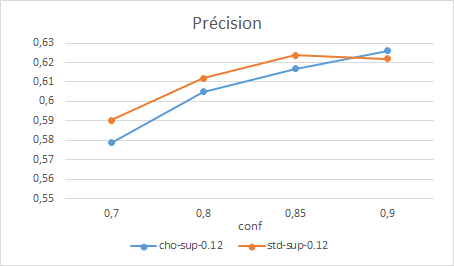
\includegraphics[height=5cm]{s0-012.png}
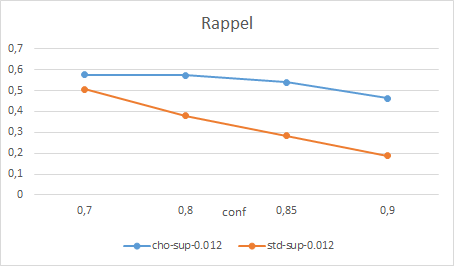
\includegraphics[height=5cm]{s0-012r.png}
\bigskip
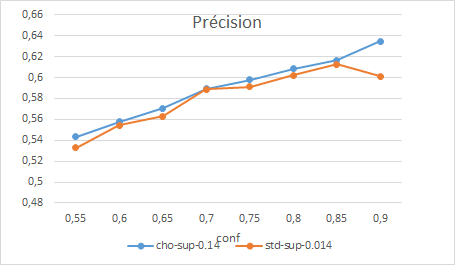
\includegraphics[height=5cm]{s0-014.png}
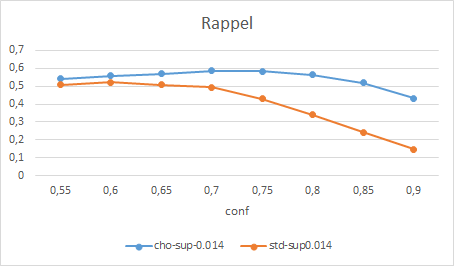
\includegraphics[height=5cm]{s0-014r.png}
\medskip
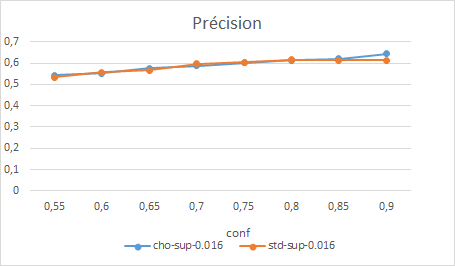
\includegraphics[height=5cm]{s0-016.png}
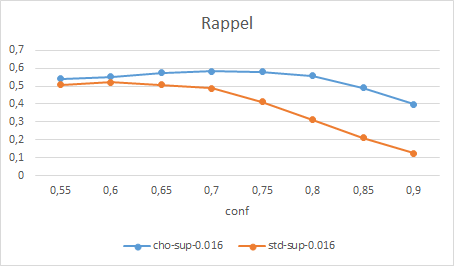
\includegraphics[height=5cm]{s0-016r.png}
\medskip
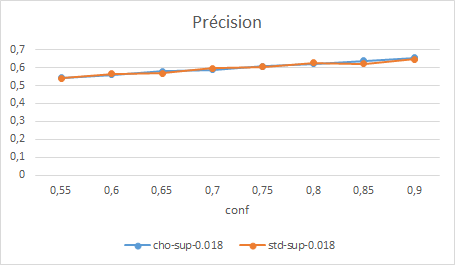
\includegraphics[height=5cm]{s0-018.png}
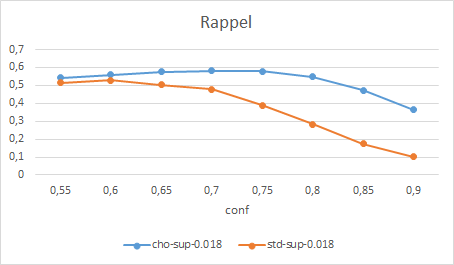
\includegraphics[height=5cm]{s0-018r.png}
\medskip
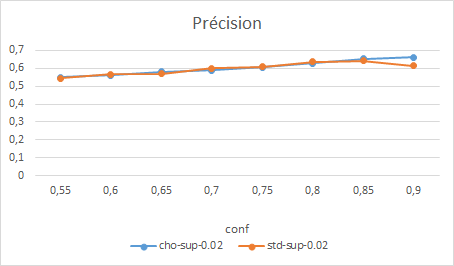
\includegraphics[height=5cm]{s0-02.png}
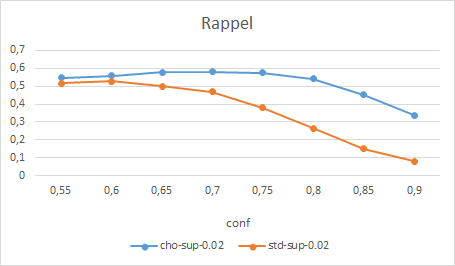
\includegraphics[height=5cm]{s0-02r.png}


\subsubsection{Interprétation}



nous pouvons passer à la phase d'implémentation qui nous permettra alors d'éffectuer une comparaison de cette approche avec l'approche de Sprex.
     \begin{center}
     
     	\begin{tikzpicture}[
     		auto,
     	        decision/.style = { diamond, draw=blue, thick, fill=blue!20,
     	                            text width=5em, text badly centered,
     	                            inner sep=1pt, rounded corners },
     	        block/.style    = { rectangle, draw=blue, thick, 
     	                            fill=blue!20, text width=10em, text centered,
     	                            rounded corners, minimum height=2em },
     	        line/.style     = { draw, thick, ->, shorten >=2pt },
     	      ]
     	      % Define nodes in a matrix
     	      \matrix [column sep=5mm, row sep=10mm] {
                      & \node [block] (PU) {Préférences utilisateur}; & \\
                      & \node [block] (TP)
                          {Transactions de préférence};            & \\
                      & \node [block] (IF)
                          {Itemsets fréquents minimaux};          & \\
                      & \node [block] (RI)
  	                            {Règles de préférence intéressantes};          & \\
     	    };
     	      % connect all nodes defined above
     	      \begin{scope} [every path/.style=line]
 	    	        \path (PU)    --    node [near start] {Algorithme 2 }
 	    	        (TP);
 	    	        \path (TP)    --    node [near start] {Algorithme 3 }
 	    	            	         (IF);
 	    	        \path (IF)    --    node [near start] {Algorithme 4 } (RI);
     	      \end{scope}
     	
     	    \end{tikzpicture}
      \end{center}
     	
     \noindent Le diagramme ci dessus énonce les différentes étapes du processus permettant l'extraction des règles de préférence intéressantes. Ces étapes seront décrites par la suite. Nous allons tout d'abord définir le support d'un itemset et la confiance d'une règle.
     
    
     
    \subsubsection{Etapes de transformation des préférences utilisateurs en transaction de préférence}
    
       Cette étape consiste à transformer le couple $<t_{1},t_{2}>$ de préférences utilisateur en une transaction de formules que l'on appellera \textbf{transaction de préférence}.\\ 
       \textbf{Principe}
       Il se fonde sur le formalisme de Chomicky appliqué aux règles de préférence contextuelles comme précédemment énoncé. Ainsi la prise en compte de la symétrie et de l'asymétrie dans cette situation, nous amène à définir ci-dessous les items élémentaires qui seront utilisés dans les transactions de préférence:\\











 
 
      \subsubsection{Etape de l'extraction des règles interressantes minimales des transactions de préférence}
 	Cette étape peut utiliser toute méthode d'extraction d'itemsets intérresaants minimaux. Notre choix s'est porté sur une méthode d'extraction des itemsets fréquents minimaux décrite dans l'article \cite{SOUL}, du faite du peu de mémoire dont elle nécessite pour l'extraction.\\
 	\textbf{Principe}\\
 	Elle consiste en un parcours en profondeur basé sur le principe du calcul des objets critiques. On a que
 	\[
 		X\in \mathcal{F}\text{ est minimal ssi }\forall e \in X,\; \widehat{cov}(X,e)\neq \emptyset
 	\]
 	avec $\widehat{cov}(X,e)=cov(X\setminus e)\setminus cov(e)$ et $cov$ étant la couverture d'un itemset (nombre de transactions contenant l'itemset). Donc à chaque ajout d'un item à un itemset $X$ lors d'un parcours en profondeur, l'évaluation de la minimalité du nouvel itemset $Y$ obtenu se fait en utilisant l'égalité suivante:
 	\[
 		 	\widehat{cov}(Xe',e)=\widehat{cov}(X,e)\cap cov(e')
 	\]
 	Ainsi il suffit d'obtenir la couverture du nouvel item ajouté pour savoir si le nouvel itemset formé est minimal.
 	
 	A partir de cette procédure, étant donné que la minimalité que nous utilisons est une minimalité basée sur le support et sur la confiance, nous allons procéder comme suit:
 	\begin{itemize}
 	 \item Générer la base de transactions de préférences inverses et ajouter celle ci à la base de préférence initiale.
 	 \item Extraire à l'aide du procédé précédent, les itemsets minimaux suivant leur support
 	 \item Filtrer les itemsets obtenus suivant que leur support dans la base initiale soit supérieur au support seuil. 
 	\end{itemize}
 		
 		Cette procédure s'explique par le fait que si un itemset $X$ est minimal dans la base globale, c'est que 
 		\[
 		\forall e\in X,\; supp(X\setminus e)\neq supp(X)\text{ ou }conf(X\setminus e)\neq conf(X)
 		\]
    
    
    
    \subsection{Algorithme}
    
 \begin{algorithm}[H]
 
 
 	\Entree{Préférences utilisateur $\mathcal{P}$}
 	\Sortie{Règles de préférence interressantes $\mathcal{R}$}
 	
 	\Deb{
 		$\mathcal{P}_{S}=\emptyset$ \tcp*[l]{Ensemble des transactions obtenues des tuples de préférence}
 		\PourCh {$<T,U>\in \mathcal{P}$}
 		{
 			$\mathcal{P}_{TU}=\emptyset$\tcp*[r]{Ensemble des items}
 			\PourCh {$A_{i} \in R$}
 			{
 				$x=T.A_{i}$ \tcp*[l]{Val correspondante à l'attribut $A_{i}$ de $T$}
 				$y=U.A_{i}$\;
 				$\mathcal{P}_{TU}=\mathcal{P}_{TU}\bigcup$ Comparaison($x,y,A_{i}$)\;
 			}
 			Ajouter ${P}_{TU}$ à ${P}_{S}$\;
 		}
 		$\mathcal{F}=$ExtraireItemsetFréquents(${P}_{S}$)\;
 		$\mathcal{R}=$FiltrerRèglesInterressantes($\mathcal{F}$)\;
 		Retourner $\mathcal{R}$\;
 	}
 	\caption{Algorithme d'extraction de règles interressantes}
 \end{algorithm}
 
 
 
 
 	
 
 
 
    
    
    \subsection{Exemple d'extraction des règles de préférence}
    Nous allons étudier deux situations:
    \begin{itemize}
    		\item Cas où le schémas relationel $\mathcal{R}(\mathcal{A}_{1},\mathcal{A}_{2},...,\mathcal{A}_{n})$ n'a que des attributs symboliques;
    		\item Cas où le schémas relationnel $\mathcal{R}(\mathcal{A}_{1},\mathcal{A}_{2},...,\mathcal{A}_{n})$ a des attributs symboliques et numériques.\\
    \end{itemize}
    
   \subsubsection{ Cas où le schémas relationnel  n'a que des attributs symboliques}
      Prenons un schémas relationnel $\mathcal{R}(\mathcal{A}_{1},\mathcal{A}_{2})$ avec $A_{1}$ et $A_{2}$ de type symboliques. Soit la base de préférence ci dessous:
      \begin{center}
      \begin{tabular}{l|l|l|l|l| } 
      
       &\multicolumn{2}{c|}{$t_{1}$} & \multicolumn{2}{c|}{$t_{2}$}\\
      \cline{2-5}
   		$P_{1}$ & a & A & b & B\\
   		$P_{2}$ & b & A & a & B\\
   		$P_{3}$ & a & A & a & B\\
   		$P_{4}$ & a & A & a & C\\
   		$P_{5}$ & b & B & a & A\\
   	\cline{2-5}
      \end{tabular}
      \end{center}   
      
        \textbf{Passage des préférences vers les transactions de préférence}\\
        On a:\\
   
        
        \noindent $P_{1}\Rightarrow T_{1}=\{C:\{x_{1}\neq y_{1}\},P:\{x_{1}=a\},N:\{y_{1}=b\},C:\{x_{2}\neq y_{2}\},P:\{x_{2}=A\},N:\{y_{2}=B\},\}$ \\
        
        \noindent $P_{2}\Rightarrow T_{2}=\{C:\{x_{1}\neq y_{1}\},P:\{x_{1}=b\},N:\{y_{1}=a\},C:\{x_{2}\neq y_{2}\},P:\{x_{2}=A\},N:\{y_{2}=B\},\}$ \\
        
        \noindent $P_{3}\Rightarrow T_{3}=\{C:\{x_{1}=y_{1}\},C:\{x_{1},y_{1}=a\},C:\{x_{2}\neq y_{2}\},P:\{x_{2}=A\},N:\{y_{2}=B\},\}$ \\
        
        \noindent $P_{4}\Rightarrow T_{4}=\{C:\{x_{1}=y_{1}\},C:\{x_{1},y_{1}=a\},C:\{x_{2}\neq y_{2}\},P:\{x_{2}=A\},N:\{y_{2}=C\},\}$ \\
        
        \noindent $P_{5}\Rightarrow T_{5}=\{C:\{x_{1}\neq y_{1}\},P:\{x_{1}=b\},N:\{y_{1}=a\},C:\{x_{2}\neq y_{2}\},P:\{x_{2}=B\},N:\{y_{2}=A\},\}$ \\
        
        
        
        \subsection{Determination des itemsets interressants minimaux avec supmin=2 et confmin=0.5}
        
        Itemsets interressants minimaux de taille 1 +++++++++++++++++++++++\\
        
        $I_{4}=\{P:\{x_{2}=A\},\}$  sup=4.0 conf=0.8\\
        $I_{5}=\{N:\{y_{2}=B\},\}$  sup=3.0 conf=0.75\\
        $I_{6}=\{P:\{x_{1}=b\},\}$  sup=2.0 conf=0.666666666667\\
        $I_{7}=\{N:\{y_{1}=a\},\}$  sup=2.0 conf=0.666666666667\\
        
        Itemsets interressants minimaux de taille 2 ++++++++++++++++++++++\
        
        $I_{14}=\{C:\{x_{1}\neq y_{1}\},P:\{x_{2}=A\},\}$  sup=2.0 conf=0.666666666667\\
        $I_{15}=\{C:\{x_{1}\neq y_{1}\},N:\{y_{2}=B\},\}$  sup=2.0 conf=0.666666666667\\
        $I_{29}=\{P:\{x_{2}=A\},C:\{x_{1}=y_{1}\},\}$  sup=2.0 conf=1.0\\
        $I_{30}=\{P:\{x_{2}=A\},C:\{x_{1},y_{1}=a\},\}$  sup=2.0 conf=1.0\\
        
        
        Pas d'itemsets interressant minimaux de taille 3\\
        
        
        
        \subsubsection{Cas où le schémas relationnel a des attributs numériques et symboliques}
        	Prenons un schémas relationnel $\mathcal{R}(\mathcal{A}_{1},\mathcal{A}_{2})$ avec $A_{1}$ et $A_{2}$ de type symboliques. Soit la base de préférence ci dessous:
        	\begin{center}
        	\begin{tabular}{l|l|l|l|l| } 
        	
        	&\multicolumn{2}{c|}{$t_{1}$} & \multicolumn{2}{c|}{$t_{2}$}\\
        	\cline{2-5}
        		$P_{1}$ & a & 3 & b & 7\\
        		$P_{2}$ & a & 3 & b & 3\\		
        		$P_{3}$ & b & 3 & a & 7\\
        		$P_{4}$ & a & 3 & a & 7\\
        		$P_{5}$ & a & 3 & a & 9\\
        		$P_{6}$ & b & 9 & a & 7\\
        		$P_{7}$ & b & 7 & a & 3\\
        	\cline{2-5}
        	\end{tabular}
        	\end{center}
        
        
        Transactions de preference obtenues\\
        
        \noindent $P_{1}\Rightarrow T_{1}=\{C:\{x_{1}\neq y_{1}\},P:\{x_{1}=a\},N:\{y_{1}=b\},C:\{x_{2}\neq y_{2}\},P:\{x_{2}=3\},N:\{y_{2}=7\},P:\{x_{2}<y_{2}\},N:\{y_{2}>3\},P:\{x_{2}<7\},C:\{x_{2},y_{2}<9\},\}$ \\
        
        \noindent $P_{2}\Rightarrow T_{2}=\{C:\{x_{1}\neq y_{1}\},P:\{x_{1}=a\},N:\{y_{1}=b\},C:\{x_{2}=y_{2}\},C:\{x_{2},y_{2}=3\},C:\{x_{2},y_{2}<7\},C:\{x_{2},y_{2}<9\},\}$ \\
        
        \noindent $P_{3}\Rightarrow T_{3}=\{C:\{x_{1}\neq y_{1}\},P:\{x_{1}=b\},N:\{y_{1}=a\},C:\{x_{2}\neq y_{2}\},P:\{x_{2}=3\},N:\{y_{2}=7\},P:\{x_{2}<y_{2}\},N:\{y_{2}>3\},P:\{x_{2}<7\},C:\{x_{2},y_{2}<9\},\}$ \\
        
        \noindent $P_{4}\Rightarrow T_{4}=\{C:\{x_{1}=y_{1}\},C:\{x_{1},y_{1}=a\},C:\{x_{2}\neq y_{2}\},P:\{x_{2}=3\},N:\{y_{2}=7\},P:\{x_{2}<y_{2}\},N:\{y_{2}>3\},P:\{x_{2}<7\},C:\{x_{2},y_{2}<9\},\}$ \\
        
        \noindent $P_{5}\Rightarrow T_{5}=\{C:\{x_{1}=y_{1}\},C:\{x_{1},y_{1}=a\},C:\{x_{2}\neq y_{2}\},P:\{x_{2}=3\},N:\{y_{2}=9\},P:\{x_{2}<y_{2}\},N:\{y_{2}>3\},N:\{y_{2}>7\},P:\{x_{2}<7\},P:\{x_{2}<9\},\}$ \\
        
        \noindent $P_{6}\Rightarrow T_{6}=\{C:\{x_{1}\neq y_{1}\},P:\{x_{1}=b\},N:\{y_{1}=a\},C:\{x_{2}\neq y_{2}\},P:\{x_{2}=9\},N:\{y_{2}=7\},P:\{x_{2}>y_{2}\},P:\{x_{2}>7\},N:\{y_{2}<9\},C:\{x_{2},y_{2}>3\},\}$ \\
        
        \noindent $P_{7}\Rightarrow T_{7}=\{C:\{x_{1}\neq y_{1}\},P:\{x_{1}=b\},N:\{y_{1}=a\},C:\{x_{2}\neq y_{2}\},P:\{x_{2}=7\},N:\{y_{2}=3\},P:\{x_{2}>y_{2}\},P:\{x_{2}>3\},N:\{y_{2}<7\},C:\{x_{2},y_{2}<9\},\}$ \\
        
        
       \newpage
       
        \subsection{Determination des itemsets interressants minimaux avec supmin=2 et confmin=0.5}
        
        Itemsets interressants minimaux de taille 1 ++++++++++++++++++++\\
        
        $I_{4}=\{P:\{x_{2}=3\},\}$  sup=4.0 conf=0.8\\
        $I_{5}=\{N:\{y_{2}=7\},\}$  sup=4.0 conf=0.8\\
        $I_{6}=\{P:\{x_{2}<y_{2}\},\}$  sup=4.0 conf=0.666666666667\\
        $I_{7}=\{N:\{y_{2}>3\},\}$  sup=4.0 conf=0.8\\
        $I_{8}=\{P:\{x_{2}<7\},\}$  sup=4.0 conf=0.8\\
        $I_{13}=\{P:\{x_{1}=b\},\}$  sup=3.0 conf=0.6\\
        $I_{14}=\{N:\{y_{1}=a\},\}$  sup=3.0 conf=0.6\\
        
        Itemsets interressants minimaux de taille 2 +++++++++++++++++++\\
        
        $I_{32}=\{C:\{x_{1}\neq y_{1}\},P:\{x_{2}=3\},\}$  sup=2.0 conf=0.666666666667\\
        $I_{33}=\{C:\{x_{1}\neq y_{1}\},N:\{y_{2}=7\},\}$  sup=3.0 conf=0.75\\
        $I_{35}=\{C:\{x_{1}\neq y_{1}\},N:\{y_{2}>3\},\}$  sup=2.0 conf=0.666666666667\\
        $I_{36}=\{C:\{x_{1}\neq y_{1}\},P:\{x_{2}<7\},\}$  sup=2.0 conf=0.666666666667\\
        $I_{74}=\{C:\{x_{2}\neq y_{2}\},P:\{x_{1}=b\},\}$  sup=3.0 conf=0.75\\
        $I_{75}=\{C:\{x_{2}\neq y_{2}\},N:\{y_{1}=a\},\}$  sup=3.0 conf=0.75\\
        $I_{79}=\{P:\{x_{2}=3\},N:\{y_{2}=7\},\}$  sup=3.0 conf=0.75\\
        $I_{83}=\{P:\{x_{2}=3\},C:\{x_{2},y_{2}<9\},\}$  sup=3.0 conf=0.75\\
        $I_{86}=\{P:\{x_{2}=3\},C:\{x_{1}=y_{1}\},\}$  sup=2.0 conf=1.0\\
        $I_{87}=\{P:\{x_{2}=3\},C:\{x_{1},y_{1}=a\},\}$  sup=2.0 conf=1.0\\
        $I_{89}=\{N:\{y_{2}=7\},P:\{x_{2}<y_{2}\},\}$  sup=3.0 conf=0.75\\
        $I_{90}=\{N:\{y_{2}=7\},N:\{y_{2}>3\},\}$  sup=3.0 conf=0.75\\
        $I_{91}=\{N:\{y_{2}=7\},P:\{x_{2}<7\},\}$  sup=3.0 conf=0.75\\
        $I_{92}=\{N:\{y_{2}=7\},C:\{x_{2},y_{2}<9\},\}$  sup=3.0 conf=0.75\\
        $I_{93}=\{N:\{y_{2}=7\},P:\{x_{1}=b\},\}$  sup=2.0 conf=1.0\\
        $I_{94}=\{N:\{y_{2}=7\},N:\{y_{1}=a\},\}$  sup=2.0 conf=1.0\\
        $I_{100}=\{P:\{x_{2}<y_{2}\},C:\{x_{2},y_{2}<9\},\}$  sup=3.0 conf=0.75\\
        $I_{103}=\{P:\{x_{2}<y_{2}\},C:\{x_{1}=y_{1}\},\}$  sup=2.0 conf=1.0\\
        $I_{104}=\{P:\{x_{2}<y_{2}\},C:\{x_{1},y_{1}=a\},\}$  sup=2.0 conf=1.0\\
        $I_{107}=\{N:\{y_{2}>3\},C:\{x_{2},y_{2}<9\},\}$  sup=3.0 conf=0.75\\
        $I_{110}=\{N:\{y_{2}>3\},C:\{x_{1}=y_{1}\},\}$  sup=2.0 conf=1.0\\
        $I_{111}=\{N:\{y_{2}>3\},C:\{x_{1},y_{1}=a\},\}$  sup=2.0 conf=1.0\\
        $I_{113}=\{P:\{x_{2}<7\},C:\{x_{2},y_{2}<9\},\}$  sup=3.0 conf=0.75\\
        $I_{116}=\{P:\{x_{2}<7\},C:\{x_{1}=y_{1}\},\}$  sup=2.0 conf=1.0\\
        $I_{117}=\{P:\{x_{2}<7\},C:\{x_{1},y_{1}=a\},\}$  sup=2.0 conf=1.0\\
        $I_{127}=\{P:\{x_{1}=b\},P:\{x_{2}>y_{2}\},\}$  sup=2.0 conf=0.666666666667\\
        $I_{130}=\{N:\{y_{1}=a\},P:\{x_{2}>y_{2}\},\}$  sup=2.0 conf=0.666666666667\\
        
        Itemsets interressants minimaux de taille 3 ++++++++++++++++++++++\\
        
        $I_{151}=\{C:\{x_{1}\neq y_{1}\},N:\{y_{2}=7\},P:\{x_{2}<y_{2}\},\}$  sup=2.0 conf=0.666666666667\\
        $I_{154}=\{C:\{x_{2},y_{2}<9\},C:\{x_{1}\neq y_{1}\},N:\{y_{2}=7\},\}$  sup=2.0 conf=0.666666666667\\
        $I_{160}=\{C:\{x_{2},y_{2}<9\},C:\{x_{1}\neq y_{1}\},P:\{x_{2}<y_{2}\},\}$  sup=2.0 conf=0.666666666667\\
        $I_{197}=\{C:\{x_{2},y_{2}<9\},C:\{x_{2}\neq y_{2}\},P:\{x_{1}=b\},\}$  sup=2.0 conf=0.666666666667\\
        $I_{198}=\{C:\{x_{2},y_{2}<9\},C:\{x_{2}\neq y_{2}\},N:\{y_{1}=a\},\}$  sup=2.0 conf=0.666666666667\\
 
        
        Pas d'itemsets interressant minimaux de taille 4\\
%Définition 16. Soient $P_x$ et 
%et  py
%deux relations de preferences sur le même schema
%relationnel R. La relation de composition pareto  px
%⊗ py
%est définie sur la relation R
%comme suit : ∀ ti, tj de R, ti  px
%⊗ py
%tj ssi (ti  px
%tj ∧¬(tj  py
%ti)) ∨ (ti  py
%tj ∧¬(tj  px
%ti)).
%Il est à noter que pour deux tuples t1  et t2  et une relation de préférence  p, ¬(t1  p
%t2) ≡ (t2  t1) ∨ (t1 ∼ p t2). De façon intuitive sous la composition pareto, un tuple t est
%préféré à un tuple u si t est au moins aussi préféré que u pour une relation de préférences
%et que t est absolument plus préféré que u pour l’autre relation de préférences.
%Exemple 11. La préférence pareto px ⊗py  (px  et py  sont définies dans l’exemple 10)
%peut être défini comme : ti  px
%⊗ py
%tj, si et seulement si, (ti   [genre] = ’drame’
%∧  tj[genre]  =
%0
%comedy
%0∧  ti[Language]  =
%0
%F rench
%0∧  tj[Language]  =
%0
%English
%0
%)∨
%(ti[Language]   =
%0
%F rench
%0∧  tj[Language]   =
%0
%English
%0∧  tj[genre]6=  ’Drame’) ∨
%(ti[Language] =
%0
%F rench
%0∧ tj[Language] =
%0
%English
%0∧ ti[genre]6= ’comedy’).
%Le modèle de préférence pareto peut être aussi appliqué sur des relations qui sont dé-
%finies sur des schémas différents [SKP11]. Soient  px
%et  py
%deux relations de préférences
%définies sur les schémas relationnels R et R
%0
%avec des domaines d’attributs dom(A) et
%dom(A’) respectivement. La relation de préférence pareto multi-dimensionnelle  px
%⊗ py
%définie sur le produit cartésien R × R’ est un sous ensemble de dom(A)× dom(A’) tel que
%(ti, t
%0
%i
%)  px
%⊗ py
%(tj, t
%0
%j
%) si et seulement si (ti  px
%tj ∧ ¬(t
%0
%j
% py
%t
%0
%i
%)) ∨ (t
%0
%i
% py
%t
%0
%j
%∧ ¬(tj  px1.1 Notion de base sur les préférences 47
%ti)) où ti  et tj  sont des tuples de R et t
%0
%i
%et t
%0
%j
%sont des tuples de R
%0
%.
%1.1.3.3  Réseaux de preferences conditionnelles (CP-nets)
%Les réseaux de préférences conditionnelles CP-nets permettent de représenter de façon
%compacte et intuitive les relations de préférences. C’est un formalisme graphique qui
%permet de modéliser les préférences conditionnelles de façon qualitative [BBD
%+
%03].
%Un CP-net sur un ensemble d’attributs A = {A1, ..., Ad } est un graphe direct dans
%lequel il existe un noeud pour chaque attribut Ai  dans A. Si une flèche d’un attribut Aj
%vers un attribut Ai  existe, alors Aj  est dit parent de Ai, on note Pa(Ai) tous les parents
%d’une variable Ai.
%Si P a(Ai) est l’ensemble des parents de Ai, les préférences sur l’attribut Ai  dépendent
%de celles sur les attributs parents de Ai  .
%Les tables de préférences conditionnelles (CPT) décrivent les préférences sur les va-
%leurs Ai  en se basant sur la combinaison des valeurs des parents de Ai.
%Une table de préférences conditionnelle de Ai, noté CPT(Ai), contient un ensemble de
%règles de préférences de la forme zi  : ai1  ai2 ; où zi ∈dom(Pa(Ai)) et ai1, ai2  appar-
%tiennent à dom(Ai).
%Ces règles de préférences sont interprétées de la façon suivante : étant donnée zi, ai1  est
%strictement préféré à ai2  (ceteris paribus).
%En d’autres termes, cette règle de préférence indique qu’un tuple contenant zi  et ai1
%est préféré à un tuple contenant zi  et ai2  ssi les valeurs des deux tuples sur les autres
%attributs sont les mêmes.
%Il est à noter que ces règles de préférences sont une spécialisation des règles de Wilson
%présentées dans la Définition 10. Il suffit de constater que dans les règles présentées par
%les CP-nets, Pa(Ai)=U et W = ∅. Nous allons ci après introduire la définition formelle
%d’un CP-net [BBD
%+
%03].
%Définition 17. Un CP-net sur les attributs A = {A1, ..., Ad } est un graphe orienté sur
%les attributs {A1, A2, ..., Ad } où chaque noeud, Ai, est annoté avec une table de préférence
%conditionnelle, CPT(Ai). Chaque table de préférence conditionnelle CPT(Ai) associe un
%ordre total  i
%zi
%pour chaque instanciation zi  de Pa(Ai).
%Exemple 12. En considérant la relation movies= {Genre, Director} tel que :
%dom(Genre)  =  {comedy, drama}  et dom(Director)  =  {W.Allen, M.Curtiz}. Consi-
%dérons l’expression de préférence suivant :
%Préférer les films de comédie aux films de drames et préférer un film dirigé par W.Allen48 Chapitre 1 : Définition des concepts
%à un film dirigé par M. Curtiz pour les films de comédie et pour les films de drames,
%préférer les films dirigés par M. Curtiz à ceux dirigés par W. Allen.
%Le CP-net correspondant à cet exemple est représenté par la figure 1.1; l’élément le
%Figure 1.1 – (a) CP-Nets correspondant aux films; (b) le graphe de préférences induit.
%plus au dessus du graphe est l’élément le moins préféré tandis que l’élément le plus en bas
%du graphe est le meilleur élément. En considérant ce CP-net, l’élément (drama,W.Allen)
%est le moins préféré tandis que l’élément (Comedy,W.Allen) est le plus préféré.
%Si on note N ce CP-net sur les attributs Genre et Director, N contient l’ensemble de
%préférences conditionnelles suivant :
%N = {comedy  drama, comedy : W.Allen  M.Curtiz, drama : M.Curtiz  W.Allen}
%Ces règles de préférence sont tout simplement les contraintes exprimées par les tables de
%préférences conditionnelles associés aux noeuds du CP-net.
%Nous allons maintenant montrer comment comparer deux transactions en utilisant un
%CP-net.
%Définition 18. Soit N un CP-net sur A, Ai ∈ A un attribut et P a(Ai) ⊂ A les parents
%de Ai  dans A. Soit Y  = A − (P a(Ai) ∪ {Ai }). Soit  i
%zi
%l’ordre sur dom(Ai) induit par
%CP T (Xi) pour chaque instanciation zi dans dom(P a(Ai)) des parents de Ai. Finalement,
%soit  une relation de préférences sur dom(A). Une relation de préférences  satisfait
% i
%zi
%ssi pour chaque y ∈dom(Y ) et chaque ai1, ai2 ∈ dom(Ai), si yai1zi  yai2zi  alors1.1 Notion de base sur les préférences 49
%ai1  i
%zi
%ai2.
%Une relation de préférences  satisfait la table de préférences conditionnelles CPT(Ai)
%ssi elle satisfait  i
%zi
%pour chaque zi  dans dom(P a(Ai)). Une relation de préférences 
%satisfait le CP-net N ssi elle satisfait CPT(Ai) pour chaque Ai.
%Un CP-net est satisfiable ssi il existe une relation de préférences  qui le satisfait.
%Par conséquent, un réseaux N est satisfait par  ssi  satisfait chaque préférence
%conditionnelle exprimée dans les tables de préférences conditionnelles de N sous les condi-
%tions ceteris-paribus. [BBD
%+
%03] montre que tout CP-net acyclique est satisfiable.
%Exemple 13. La relation de préférences  qui induit l’ordre :{comedy ∧ W.Allen 
%comedy ∧ M.curtiz  drama ∧ M.curtiz  drama ∧ W.Allen} est la seule qui satisfait
%le CP-net de la figure 1.1.
%L’implication dans les CP-net est définie de la façon standard.
%Définition 19. Soit N un CP-net sur A et ti,tj ∈  dom(A) deux tuples, N implique
%ti  tj  (i.e que l’objet ti  est préféré à tj) noté N |= ti  tj  ssi ti  tj  est vrai dans toute
%relation de préférence qui satisfait N.
%Exemple  14. Le CP-net de la figure 1.1 implique que comedyW.Allen    
%comedyM.Curtiz puisque Cette préférence est vraie dans la seule relation de préférence
%qui satisfait le CP-net.
%Les préférences exprimées en utilisant le formalisme des CP-nets sont des préférences
%conditionnelles sous l’hypothèse ceteris paribus. La préférence exprimée sur la valeur d’un
%attribut dépend de la valeur d’autres attributs; avec les CP-nets,
%il n’y a pas de préférences contradictoires : il n’est pas possible d’appliquer deux règles
%en même temps.
%Néanmoins, le pouvoir d’expression des CP-nets est limité, il n’est pas possible de repré-
%senter toutes les préférences. Cependant, pour les utilisateurs, il est plus facile d’utiliser
%le principe ceteris paribus.
%Le formalisme proposé par Wilson [Wil04] constitue une extension des CP-nets, ce for-
%malisme permet de manipuler des expressions plus générales. Pour rappel, les règles de
%Wilson sont sous la forme u : x  x
%0
%[W ] (cf. Définition 10). Il est montré que ces expres-
%sions généralisent celles des CP-nets qui sont obtenues si W= ∅.
%En considérant l’exemple suivant :
%Exemple 15. Préférer les films de comédies aux films de drames sans tenir compte du
%directeur du film.50 Chapitre 1 : Définition des concepts
%Cette expression de préférence n’est pas représentable avec les CP-nets puisqu’ils uti-
%lisent le principe du ceteris paribus. Par contre en utilisant le formalisme de Wilson, cette
%préférence peut être représentée de la façon suivante. > : comedy  drame[Director].
%
%\textbf{Formulation de Werner Kießling}
%
%		
%\end{defn}
%
%
%Nous distinguons deux grandes approches pour représenter les préférences utilisateur: 
%\begin{itemize}
%\item L'approche quantitative
%\item l'approche qualitative
%\end{itemize}

	\bibliographystyle{plain}
	\bibliography{../biblio}




\end{document}



